\documentclass{sigplanconf}

\usepackage{makeidx}  

\usepackage{amsmath}
\usepackage{amssymb}
\usepackage{graphicx}
\usepackage{multirow}
\usepackage{tabularx}
\usepackage{paralist}

\usepackage[utf8x]{inputenc}
\usepackage{url}

\usepackage{ifthen}
\newboolean{showcomments}
\setboolean{showcomments}{false} 
\ifthenelse{\boolean{showcomments}}
	{	\newcommand{\nbnote}[2]{
			\fbox{\bfseries\sffamily\scriptsize#1}
			{\sf\small$\blacktriangleright$\textit{#2}$\blacktriangleleft$}
		}
		\newcommand{\svnversion}{
			\emph{\scriptsize$-$Id: main.tex 5044 2006-12-20 22:57:51Z hirschfeld $-$}
		}
	}
	{	\newcommand{\nbnote}[2]{}
		\newcommand{\svnversion}{}
	}
\newcommand\bs[1]{\nbnote{Bastian}{#1}}

\usepackage{todonotes}

\newcommand\slightspace{\kern0.5em}
\newcommand\hairspace{\ifmmode\mskip1mu\else\kern0.08em\fi}
\usepackage{xspace}
\newcommand{\coexist}{CoExist\xspace}
\newcommand{\eg}{e.\hairspace{}g.,\xspace}
\newcommand{\Eg}{E.\hairspace{}g.,\xspace}
\newcommand{\Ie}{I.\hairspace{}e.,\xspace}
\newcommand{\ie}{i.\hairspace{}e.,\xspace}
\newcommand{\cf}[1]{cf.\ {#1}\xspace}

\newcommand{\mydescriptionlabel}[1]{\hspace{\labelsep}\itshape{#1}}
\let\descriptionlabel\mydescriptionlabel

\usepackage{textcomp}
\usepackage{xcolor}
\usepackage{listings}

\usepackage{pifont}
\newcounter{dingdistance}
\setcounter{dingdistance}{191}
\newcommand{\circnum}[1]{%
  \addtocounter{dingdistance}{#1}%
  \ding{\value{dingdistance}}%
  \setcounter{dingdistance}{191}}

\usepackage[acronym]{glossaries}
\newcommand{\ac}[1]{\gls{#1}}
\newcommand{\acp}[1]{\glspl{#1}}
\newcommand{\Acp}[1]{\Gls{#1}}
\newacronym{api}{\textsc{api}}{application programming interface}
\newacronym{dsl}{\textsc{dsl}}{domain specific language}
\newacronym{vm}{\textsc{vm}}{Virtual Machine}
\newacronym{dom}{\textsc{dom}}{Document Object Model}
\newacronym{http}{\textsc{http}}{Hyper-text transfer protocol}
\newacronym{stm}{\textsc{stm}}{software transactional memory}
\newacronym{cop}{\textsc{cop}}{context-oriented programming}
\newacronym{vcs}{\textsc{vcs}}{Version Control System}

\usepackage{hyperref}
\def\sectionautorefname{Section}
\def\subsectionautorefname{Section}
\def\subsubsectionautorefname{Section}
\def\tableautorefname{Table}
\def\figureautorefname{Figure}

\definecolor{source}{gray}{0.95}

\lstdefinelanguage{JavaScript}{
  keywords={typeof, new, true, false, catch, function, return, null, catch, switch, var, if, in, while, do, else, case, break},
  keywordstyle=\bfseries,
  ndkeywords={class, export, boolean, throw, implements, import, this},
  ndkeywordstyle=\color{darkgray}\bfseries,
  identifierstyle=\color{black},
  sensitive=false,
  comment=[l]{//},
  morecomment=[s]{/*}{*/},
  commentstyle=\color{purple}\ttfamily,
  stringstyle=\ttfamily,
  morestring=[b]',
  morestring=[b]"
}
\lstset{%
    language=JavaScript,%
    basicstyle=\small\ttfamily,
    frame=none,%
    numbers=left,
    numbersep=5pt,
    numberstyle=\tiny\color{gray},
    stepnumber=1,
    emph={always, once, constructor},%
    emphstyle=\bfseries,%
    breakatwhitespace=false,%
    literate={<<}{\tiny{$\ll$}~}{1},%
    showstringspaces=false,%
}

\lstnewenvironment{code}[1][]%
{\vskip0em\noindent
  \minipage{\linewidth}
  \lstset{%
    language=JavaScript,%
    basicstyle=\scriptsize\ttfamily,
    frame=none,%
    numbers=left,
    numbersep=5pt,
    numberstyle=\tiny\color{gray},
    stepnumber=1,
    emph={always, once, constructor},%
    emphstyle=\bfseries,%
    breakatwhitespace=false,%
    literate={<<}{\tiny{$\ll$}~}{1},%
    showstringspaces=false,%
    columns=flexible,%
    #1}}
{\endminipage\vspace{0.25\baselineskip}}

\newcommand{\ct}{\lstinline[basicstyle={\ttfamily}]}

\newtheorem{highlight}{Highlight}

\newfont{\mycrnotice}{ptmr8t at 7pt}
\newfont{\myconfname}{ptmri8t at 7pt}
\let\crnotice\mycrnotice%
\let\confname\myconfname%

\begin{document}

\exclusivelicense
\conferenceinfo{DLS~'14}{October 20--24, 2014, Portland, OR, USA}
\copyrightyear{2014}
\copyrightdata{978-1-4503-3211-8/14/10}
\doi{10.1145/2661088.2661093}

\title{Object Versioning to Support Recovery Needs} 
\subtitle{Using Proxies to Preserve Previous Development States in Lively}

\authorinfo{Bastian Steinert \and Lauritz Thamsen \and Tim Felgentreff
  \and Robert Hirschfeld}
           {Software Architecture Group\\ Hasso Plattner Institute\\ University of Potsdam, Germany\\}
           {firstname.lastname@hpi.uni-potsdam.de}

\maketitle

\markboth{Draft of \today, submitted to ECOOP 2012}{Draft of \today, submitted to ECOOP 2012}

\begin{abstract}
  We present object versioning as a generic approach to preserve
  access to previous development and application states. Version-aware
  references can manage the modifications made to the target object
  and record versions as desired. Such references can be provided
  without modifications to the virtual machine. We used proxies to
  implement the proposed concepts and demonstrate the Lively Kernel
  running on top of this object versioning layer. This enables Lively
  users to undo the effects of direct manipulation and other programming
  actions.
\end{abstract}

\urlstyle{tt}
 % content/1_introduction.tex
\section{Introduction} 
\label{sec:INTRODUCTION}

Continuous versioning of development states provides an approach to
deal with recovery needs that is complementary to best practices to
avoid such recovery needs. Continuous versioning such as
provided by \coexist~\cite{Steinert2012COE} implicitly records
current snapshots of the development state and provides users access
to these recorded versions. Similar to undo/redo mechanisms, it runs
in the background and requires no explicit control of the
user. Similar to \acp{vcs}, it records the state of all development
artifacts at a given point in time. Finding previous versions becomes
feasible by aligning the versioning with the structure of the program
so that each recorded version represents an addition, removal, or
modification of program elements such as methods and classes. This
structured form of continuous versioning, which is the foundation of
\coexist, allows to identify previous versions based on the names of
program elements. \coexist has been proposed as a complement to
undo/redo mechanisms and explicit commits using \acp{vcs}.

While typically unanticipated recovery needs involve tedious and
time-consuming work, \coexist makes recovery tasks fast and easy to
accomplish. It helps users going back to previous devevelopment states
even if explicit commits are missing. It also supports detecting those
changes that introduced undesired behavior even if testing has been
ignored during development. With the additional support for knowledge
recovery and re-assembling changes to commits, programmers have to
spend less effort on trying to avoid unanticipated recovery needs.

However, the current prototype has revealed two main limitations, in
particular for live programming systems such as
Squeak/Smalltalk~\cite{Ingalls1997Squeak} or the Lively
Kernel~\cite{Ingalls2008LKS}. First, the current mechanism only records
versions of meta-objects such as classes and methods. This means, a
version consists of a set of classes and their methods at a particular
point in time. But besides classes and methods, systems such as Squeak
also consist of global state captured in class-side or global
variables. Global state implies direct or indirect references to
particular versions of classes in the system, which easily introduces
inconsistencies. Trying to avoid inconsistencies would make the current
versioning mechanism overly complex, which suggests, for the sake of
simplicity, the need for a different solution.

\begin{figure}
    \centering
    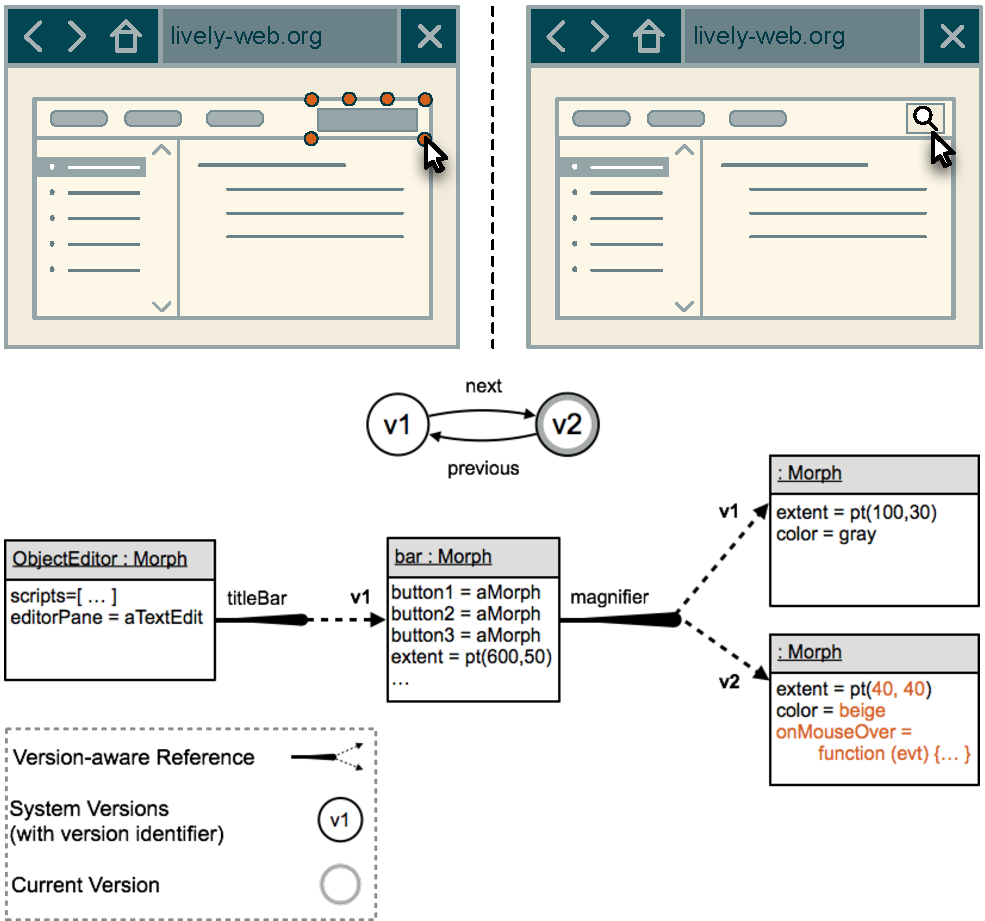
\includegraphics[width=\columnwidth]{figures/figure1_new}
    \caption{Two versions of a Lively Kernel site. Below is an excerpt
      of the corresponding object graph that provides access to both
      versions.}
    \label{fig:fig1}
\end{figure}

Second, programming often involves steps that are different from
editing source code. For example, programming can involve the
composition of visual elements such as in Etoys~\cite{Kay2005Etoys},
Scratch~\cite{Maloney2010SPL}, or Fabrik~\cite{Ingalls1988FVP}. It can
also involve the creation and manipulation of individual objects such
as in Self and Lively. Users can directly manipulate the visual
appearance of objects and modify their behavior as illustrated in the
top of \autoref{fig:fig1}. So, graphical composition and direct
manipulation are often an inherent part of programming. Furthermore,
objects are not necessarily defined by classes and may only be
anchored through visual elements.

As a consequence of the above, we conclude that a generic approach to
continuous versioning of development states should not rely on the
modification of classes and methods. The versioning mechanism should
capture the entire system state including all object state. This would
allow to record all kinds of programming actions and provide access to
previous states of the entire system. With that, undesired effects of
direct manipulation and evaluating code snippets could easily be
undone, among others.

For this reason, this paper presents object versioning as an improved
and generic approach for continuously recording development states. Object
versioning relies on alternative references that can manage multiple
versions of the target object depending on the currently active
version (\autoref{fig:fig1}). Such version-aware references can be
realized by means of proxies in order to avoid modifications of the
execution platform. We have implemented the proposed concept in
JavaScript using ECMAScript 6 proxies. Source transformations ensure
that for every mutable object a corresponding proxy is created. Besides
checking our implementation with the Octane benchmark suite, it has been
advanced and refined to have it run inside the Lively Kernel system. It is
now possible to record development states of a Lively system and go back to
previous states as desired.

The use of such a generic versioning mechanism is not restricted to
programming scenarios. It will be useful for all applications and
tools in the Lively system. Users could implicitly rely on undo/redo
and versioning facilities in various situations, for example, when they
author content of Lively Wiki pages or prepare slides using Lively's
presentation tool.

With that, this paper makes the following contributions:
\begin{itemize}
\item We present an approach to object versioning using proxies, which
\item provides an advanced generic approach to preserve access to
  previous development states, and
\item allows for scoping and rolling back the effect of programming
  actions.
\item We present an implementation using ECMAScript 6 proxies and
  document various corner cases and limitations.
\item An evaluation shows the strong performance penalties of the
  current implementation of ECMAScript 6 proxies. 
\end{itemize}


 % content/2_background.tex
\section{Background} 
\label{sec:background}
First, this section provides a summary of \coexist{}, which
provides recovery support for class-based object-oriented
programming. Second, this section illustrates programming
by means of direct manipulation and object scripting in Lively Kernel,
for which an improved generic approach to recovery support is
desirable.

\subsection{\coexist}

\begin{figure}
    \centering
    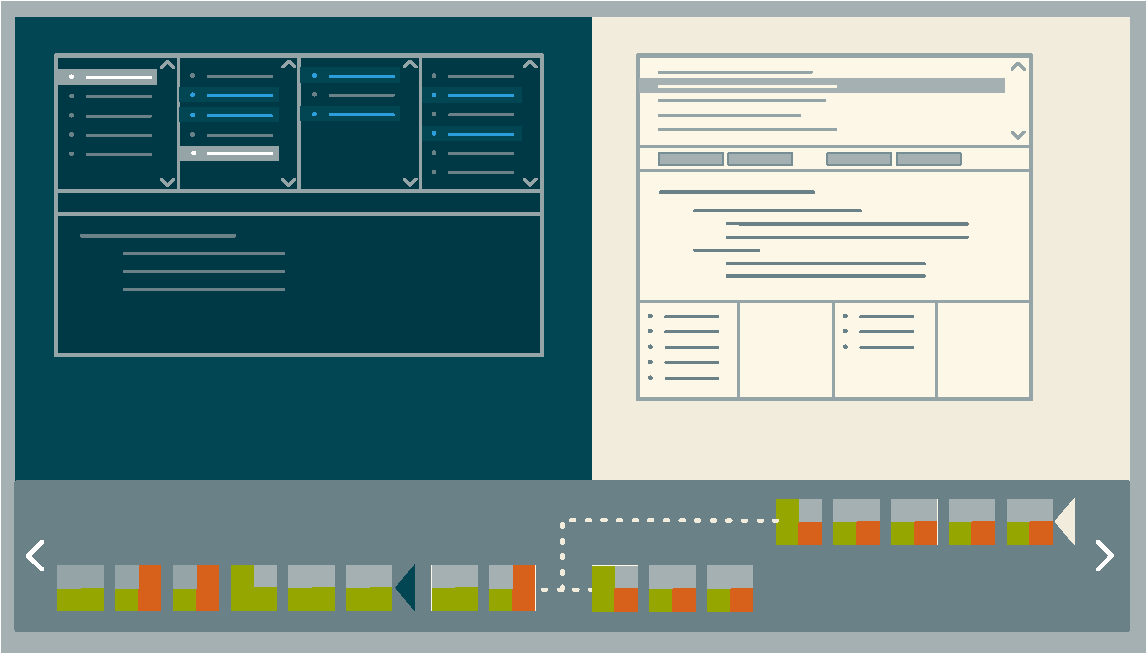
\includegraphics[width=\columnwidth]{figures/2_background/coexist2}
    \caption{Conceptual figure of \coexist featuring continuous
      versioning, running tests and recording the results in the
      background, and side by side exploring and editing of multiple
      versions.}
    \label{fig:CoExist}
\end{figure}

\coexist preserves fast and easy access to previous development
states~\cite{Steinert2012COE}. It is based on the insight that the
risk for tedious recovery is caused by the loss of immediate access to
previous development states. With every change, the previous version
is lost, unless it has been saved explicitly. This version, however,
can be of value in future development states, when, for example, an
idea turns out inappropriate. For that reason, \coexist creates a new
version for every change to the code base. Users can rapidly switch
versions or can access multiple versions next to each other. \coexist
thus gives users the impression that development versions
\emph{co-exist}. \autoref{fig:CoExist} illustrates some of the main
user interfaces concepts of \coexist. It contributes the following
concepts and tools:

\begin{description}
\item[Continuous Versioning] creates new versions in the background
  based on the structure of programs. It enables programmers to go
  back to a previous development state and to start over, which will
  implicitly create a new branch of versions.
 
\item[User Interface Concepts] support browsing and exploring version
  information as well as identifying a version of interest fast. Two
  different tools are provided. First, the version bar highlights
  version items that match the currently selected source code
  element. Hovering over the items will display additional information such
  as the kind of modification, the affected elements, or the actual
  change performed. Second, the version browser allows for exploring
  multiple versions at a glance. The version browser displays basic
  version information in a table view, which allows for scanning the
  history fast.

\item[Additional Environments] to explore static and dynamic
  information of previous development states next to the current set
  of tools. Opening an additional environment is useful, when, for
  example, the programmer becomes curious about how certain
  parts of the source code looked previously or how certain effects
  were achieved. The additional environments also allow for running
  and debugging programs. With that, users are capable of efficiently
  recovering knowledge from previous versions, which avoids the need
  for a precise understanding of every detail before making any
  changes.

\item[Continuous and Back-in-time Analysis] for test cases and other
  computations. \coexist{} continuously runs analysis programs for
  newly created versions. As a default, it runs test cases to
  automatically assess the quality of the change made. The test result
  for a version is recorded and presented in the corresponding item
  of the version bar (left of \autoref{fig:CoExist}). The user can
  also run other analyses such as performance measurements. In
  addition to the continuous analysis features, \coexist provides full
  access to version objects and offers a programming interface to run
  code in the context of a particular version. So, whenever
  programmers become interested in the impact of their changes, they
  can easily analyze them in various respects. This allows programmers
  to ignore these aspects of programming at other times.

\item[Re-assembling of Changes] for sharing independent improvements
  in separate commits. Users can extract selected changes to a new
  branch, test the result, and commit the achieved increment.
\end{description}

With \coexist, programmers can change source code without worrying
about the possibility of making an error. They can rely on tools that
will help with whatever their explorations will turn up. They no
longer have to slavishly follow certain best practices in order to keep recovery
costs low.

\subsection{Part Development in Lively Kernel}
We first describe the Lively Kernel and the Morphic framework before
we describe an example development scenario using Parts, direct
manipulation, and object scripting.

\subsubsection{The Lively Kernel and Morphic}
The Lively Kernel is a pure-JavaScript programming system in the
tradition of Smalltalk and Self and provides ideas from these systems
in a pure JavaScript environment. Development happens at runtime.  It
incorporates tools and techniques to be completely self-sufficient.
Thus, programmers can create versions of the Lively Kernel with the
Lively Kernel. The Lively Kernel is a browser-based system.  It is
implemented in JavaScript and renders to HTML.

The Lively Kernel implements Morphic~\cite{Maloney1995Mor}, a
framework for developing graphical applications.  The graphical
objects of this framework are called \emph{Morphs}. Each morph has a
class but can also have object-specific behavior. They can be created
by instantiating a class or by copying an existing morph. (Class-based
and prototype-based programming is mixed.) The copy operation does not
establish a prototypical inheritance relationship between the copy and
the original. Instead, it creates a full copy.

Programmers can change the position of morphs by \emph{dragging} and
the composition by an alternative dragging, called \emph{grabbing}.
When a morph is grabbed, it can be added to another morph and becomes
that morph's submorph.  This way, a morph does not have to be a basic
shape or simple widget, but can be the interface of any application.

\begin{figure}
    \centering
    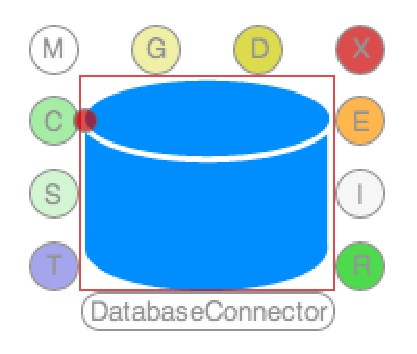
\includegraphics[width=0.3\columnwidth]{figures/2_background/1_halos.pdf}
    \caption{The halo buttons of a basic morph.}
    \label{fig:Halos}
\end{figure}

Morphs offer manipulation tools called \emph{Halos}
(\autoref{fig:Halos}). Halos enable direct manipulation of
morphs. Using halos, users can resize, rotate, drag\&drop, and copy
morphs. They can also change morph compositions by adding or removing
morphs as submorphs. Other halo buttons open tools such as an
\emph{Inspector}, \emph{Style Editor}, and \emph{Object Editor}. While
the inspector focuses on presenting all fields and values of each
object, the object editor provides means to browse and edit
object-specific scripts.

The Lively Kernel uses a \emph{Parts Bin}~\cite{Lincke2012LPC} to save
and publish morphs and morph compositions with associated behavior as
\emph{parts}.  Users can use such published parts for their own
compositions and publish their creations to the PartsBin. Various
Lively tools (such as the Object Editor) have been created and made
available by incrementally composing morphs and adding behavior that
users considered useful during development, and then publishing these
as self-contained \emph{parts}.

\subsubsection{Part Development By Example}

To exemplify how developers work directly on objects in the Lively
Kernel, we will outline how a user added a magnifier tool to the
Object Editor.  The magnifier tool helps users find the object in the
scene graph that is currently selected for editing. Implementing the
new feature requires to create a new button morph and to add it to the
editor.

\begin{figure}
    \centering
    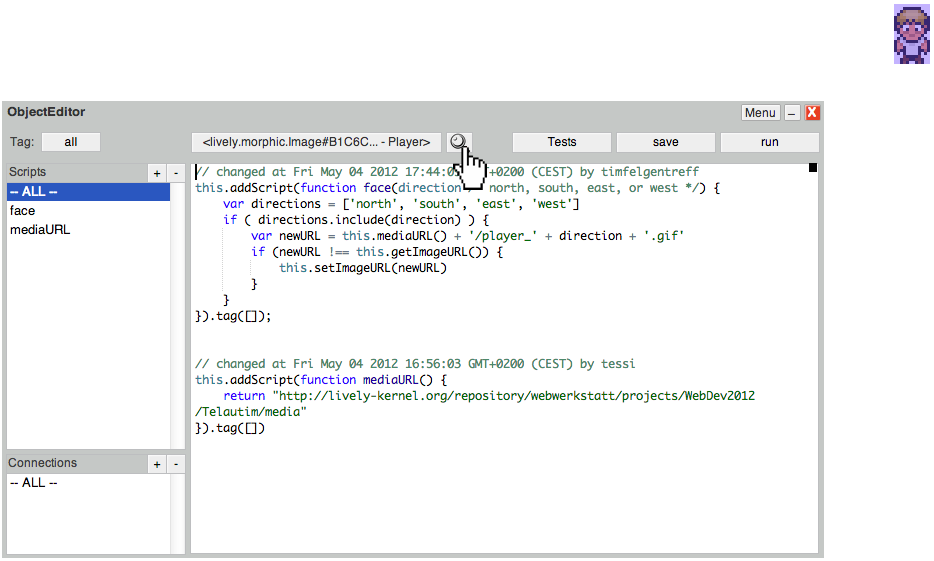
\includegraphics[width=\columnwidth]{figures/3_motivation/2_magnifierBehavior.png}
    \caption{The Object Editor's magnifier button as it highlights the editor's target.}
    \label{fig:MagnifierBehavior}
\end{figure}

The following functionality is provided by the magnifier button: When
hovering over the button, the Object Editor's current target is
highlighted with a rectangular overlay, as shown in
\autoref{fig:MagnifierBehavior}.

To add such a button, a user would first create the button and adapt
its visual appearance as shown in \autoref{fig:ButtonBuilding}. The
user can start with a basic button (\circnum{1}), which can be found
in the Parts Bin repository. In step \circnum{2}, the user resizes the
button and gives it a square extent using the \emph{Resize} halo tool.
Next, the user loads an image showing a magnifier icon (for example,
by dropping such an image onto the Web page.), and adds it to the
button using drag and drop (\circnum{3}).  Dropping a morph
onto another connects the two morphs, making the former a submorph of
the latter. Moving the button around will then move the image
accordingly. Finally, the users adds the result of these
manipulations, visible in \circnum{4}, to the Object Editor.

Note how all these changes are directly made to actual objects: the
button morph, the magnifier image morph, and the editor morph. Users
can immediately see the effects of their actions.

\begin{figure}
  \centering
    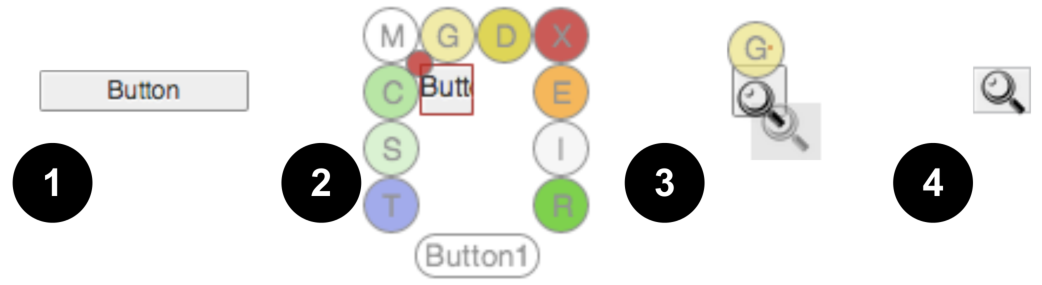
\includegraphics[width=\columnwidth]{figures/3_motivation/3_buildingTheButton.pdf}
    \caption{Directly manipulating a button morph.}
    \label{fig:ButtonBuilding}
\end{figure}

As the next step, a user would implement the button's behavior. The
user adds scripts to the button that adds a translucent rectangle over
the current target on hover.  In particular, the button receives two
scripts: \lstinline{onMouseMove} and \lstinline{onMouseOut}.  The
implementation of the behavior includes the following:

\begin{itemize}
\item The button holds a semitransparent rectangle morph.
\item When the mouse enters the button (\lstinline{onMouseMove}), the
  button resizes and adds the rectangle to the Lively Kernel world at
  the position of the target.
\item When the mouse leaves the button (\lstinline{onMouseOut}), the
  button removes the rectangle from the world again.
\end{itemize}

While developing the script, the Lively Kernel's scripting tools allow
to evaluate code in the context of their target objects.  Hence, when
programmers want to test a script or even just specific lines of code,
they can try the behavior directly for the actual target.

\subsubsection{Recovery Needs When Developing Parts}

When programmers advance the system through direct manipulation and
object scripting, they will encounter recovery needs that are
different from those possible when editing descriptions of classes and
methods:

\begin{description}
\item[Accidental changes to state] The user could accidentally grab
  and move a morph such as the new button and, thereby, change a
  carefully arranged layout. Similarly, meaningful state can be lost
  when a morph is accidentally removed from the world.
\item[Inappropriate changes through direct manipulation] The user
  could make changes to the size, position, and colors of morphs to
  fine-tune their visual appearance, only to decide later that an
  intermediate version was most appealing.
\item[Accidental changes to scripts] The user could introduce typos
  to scripts or accidentally remove a script. Moreover, editing a
  script could introduce bugs.
\item[Inappropriate changes through scripts] The user could
  make a mistake in a workspace snippet that is intended to manipulate
  morph properties programmatically. Such a snippet can change many
  properties of many objects.
\end{description}

Undesirable changes can also be introduced when users evaluate scripts
to gain feedback on their effect. For example, a user might explore
the button's \lstinline{onMouseMove} script and therefore evaluate a
few lines of code to test it.  However, while developing the script it
might not check all necessary conditions before adding the
highlighting rectangle -- for example, the developer might have
forgotten that only one highlight rectangle should be visible at a
time, so before adding a new highlight, the old one should be
deleted. Therefore, evaluating code during development can leave the
system in an inconsistent state.
The programmer than has to manually recover from that state.

These development steps show that there are many situations in which
the user might want to undo previous actions.  In programming systems
like the Lively Kernel, where programmers work on objects, changes are
always made to the state of objects. When the state of all objects is
preserved and can be re-established, previous system states can be
recovered when necessary.


 % content/4_approach.tex
\section{Object Versioning} \label{chapter:APPROACH}

A previous version of an object is, in the simplest case, a copy of
the object before its state was manipulated. The left hand side of
\autoref{fig:VersionPreserved} shows an object representing an address
with fields for \lstinline{street}, \lstinline{number}, and
\lstinline{city}. As the user interacts with the object, its state
changes and different \emph{versions} (i.e., co-existing copies) of
the object are created (\autoref{fig:VersionPreserved}).  The two
objects have no additional information to indicate to which version of
the system they belong, nor do they store any information showing that
one is a copy of the other.

\begin{figure}[h]
    \centering
    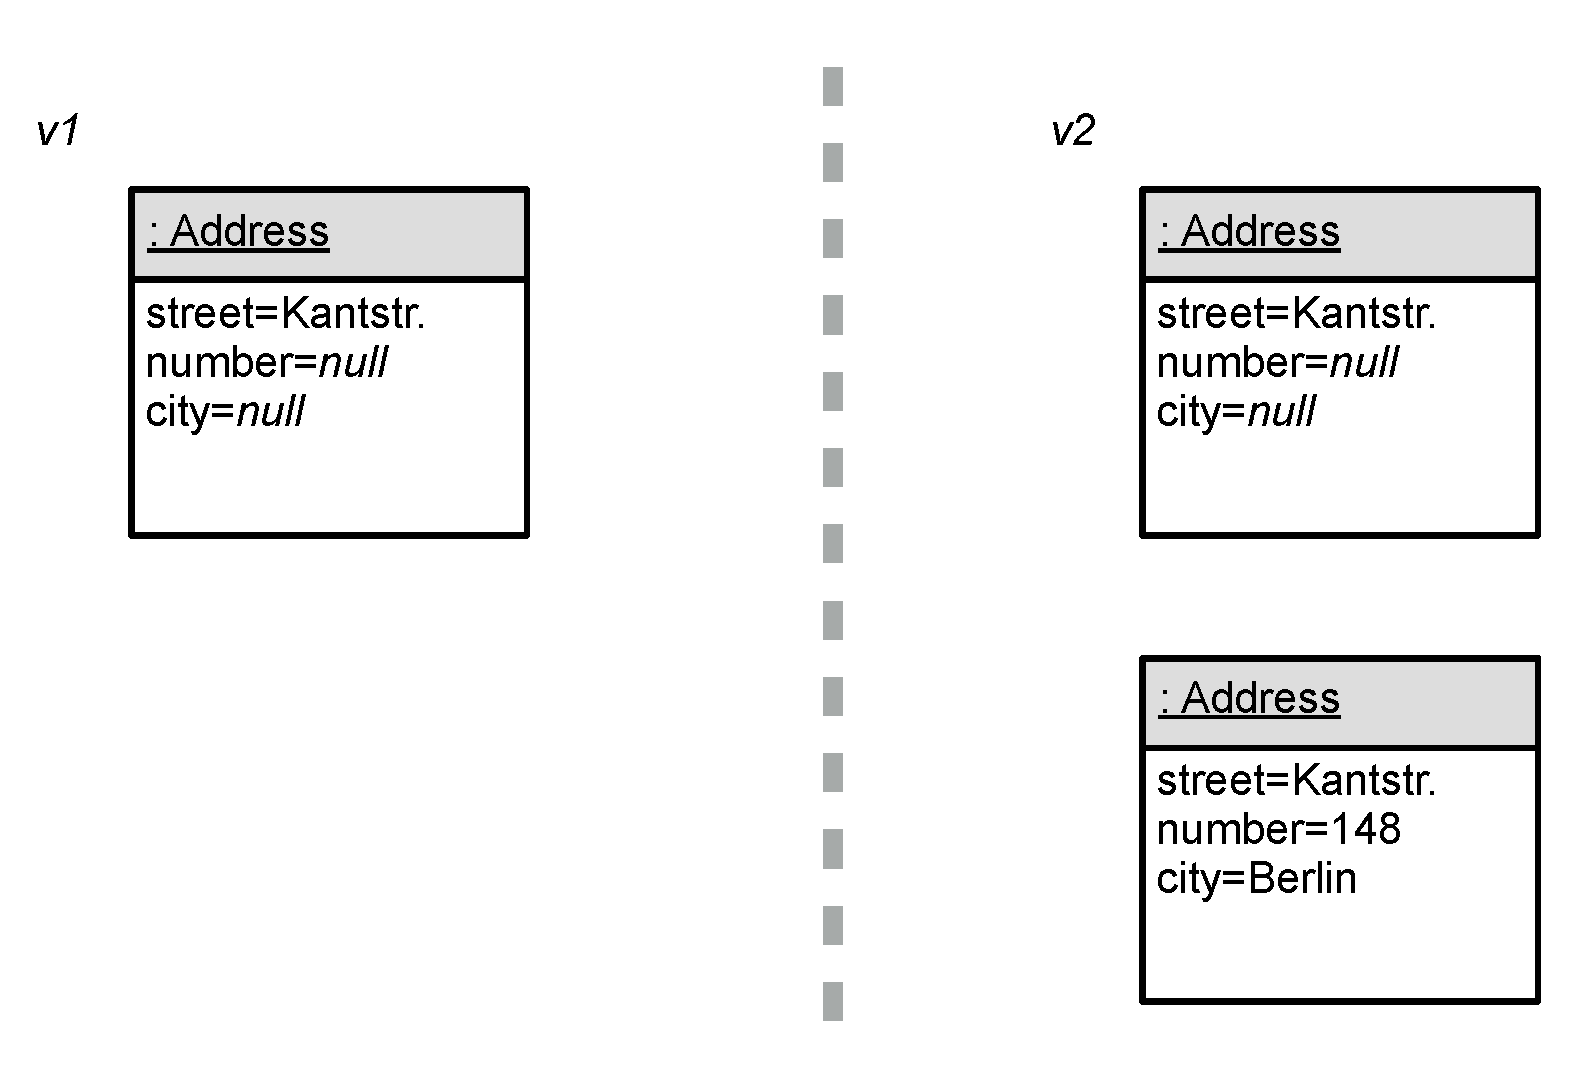
\includegraphics[width=0.7\columnwidth]{figures/4_approach/3_previousVersionPreserved.pdf}
    \caption{Preserving the previous version of the \lstinline{address} object.}
    \label{fig:VersionPreserved}
\end{figure}

To be able to access different versions of an object, its previous
states need to be kept alive through \emph{version-aware references}.
Version-aware references act like ordinary references, but also
manage the versions of an object and always resolve to one of those
based on context information. When, for example, a person object has
an \lstinline{address}, the version-aware reference resolves to either
\emph{v1} or \emph{v2} of the address, as shown in
\autoref{fig:VersionAwareReferenceFollowingVersion2}.

\begin{figure}[h]
    \centering
    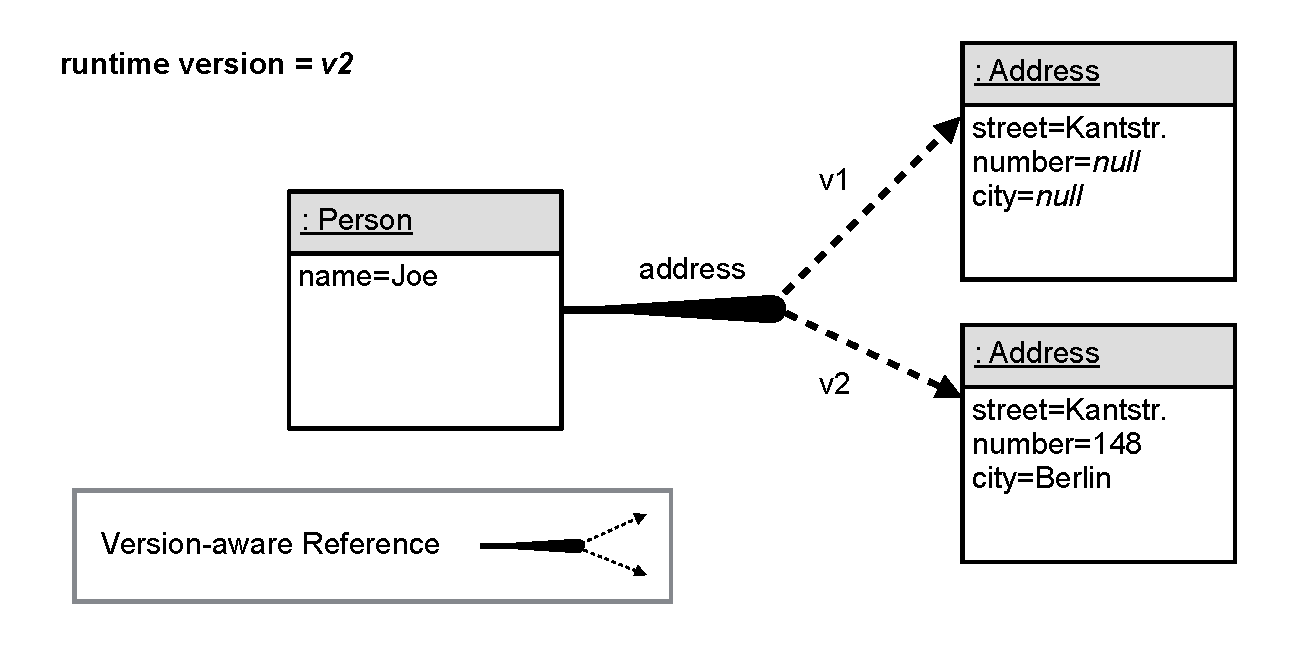
\includegraphics[width=0.8\columnwidth]{figures/4_approach/5_versionAwareReferenceFollowingVersion2.pdf}
    \caption{A version-aware reference relates a \lstinline{person} object to two versions of its \lstinline{address} property.}
    \label{fig:VersionAwareReferenceFollowingVersion2}
\end{figure}

In the same way, multiple version-aware references are resolved by
traversing an object graph. Through different possible traversals of
the version-aware object graph, different versions of the system
emerge.  All version-aware references within a traversal delegate to
versions of objects that belong to the same system state.
\autoref{fig:ObjectGraphWithReferencesResolvedAlongVersion2} shows
such an object graph.

\begin{figure}[h]
    \centering
    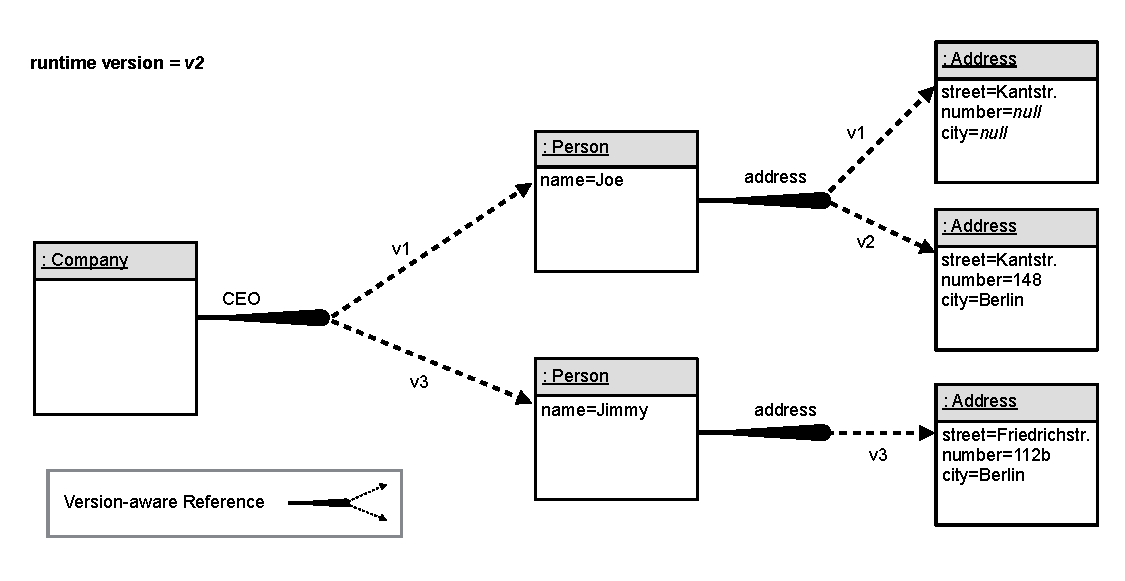
\includegraphics[width=\columnwidth]{figures/4_approach/6_objectGraphWithVersonAwareReferences.pdf}
    \caption{An object graph with version-aware references.}
    \label{fig:ObjectGraphWithReferencesResolvedAlongVersion2}
\end{figure}

\subsection{Versions of the System}
\label{sec:versions-system}

To establish system versions from version-aware object graphs, the version-aware references resolve to different object versions dynamically based on a \emph{version identifier}.
As this identifier changes, the version-aware references resolve to other versions of objects.
In order to undo a change made in version \emph{v2} of the system, the version identifier is simply set back to \emph{v1}.

Given the example situation from \autoref{fig:ObjectGraphWithReferencesResolvedAlongVersion2}, the following statement would refer to three different values depending on the version identifier:

\begin{code}
Company.CEO.address.number
\end{code}

Evaluating the statement in version \emph{v1} would return the value \lstinline{null}, in version \emph{v2} the value \lstinline{148}, and in version \emph{v3} the value \lstinline{112b}.
Note that no \emph{v2} reference exists from \lstinline{Company} to a \lstinline{ceo}.
Version identifiers have a \emph{predecessor} and a \emph{successor}, so when no current version is available, the most recent available version can be found.
This optimization allows to only create new versions of objects when necessary.

The version identifier needs to be accessible to the version-aware references.
It might be a global (to have a single active version of the system), but could also be thread-local, or in the dynamic scope of an execution.
However, it must not be changed while a versioned object graph is traversed.
This is automatically true only for dynamically scoped version identifiers.

To enable our approach to actually re-establish a particular version of the system with our approach, all mutable objects must only be accessed via version-aware references. To satisfy this requirement, we propose a system transformation that uses proxy objects as references.

\subsection{Ubiquitous Proxies as Version-aware References} \label{sec:APPROACH:2}

Applications written in JavaScript typically have to work on a variety of client \acp{vm} included in different Web browsers.
This makes a language-level implementation preferable to an implementation of \emph{alternative references} in each JavaScript \ac{vm}\@.
We use proxies pointed to by \emph{ordinary references} to delegate to object versions transparently, as shown in \autoref{fig:ProxyBasedVersionAwareReference}.
Each property accessed on a proxy is forwarded transparently to the correct version of the object.
Thus, proxies in this design are \emph{virtual objects}~\cite{VanCutsem2010PDP}; they do not stand in for a specific object, but can forward intercepted interactions to any object.

\begin{figure}[h]
    \centering
    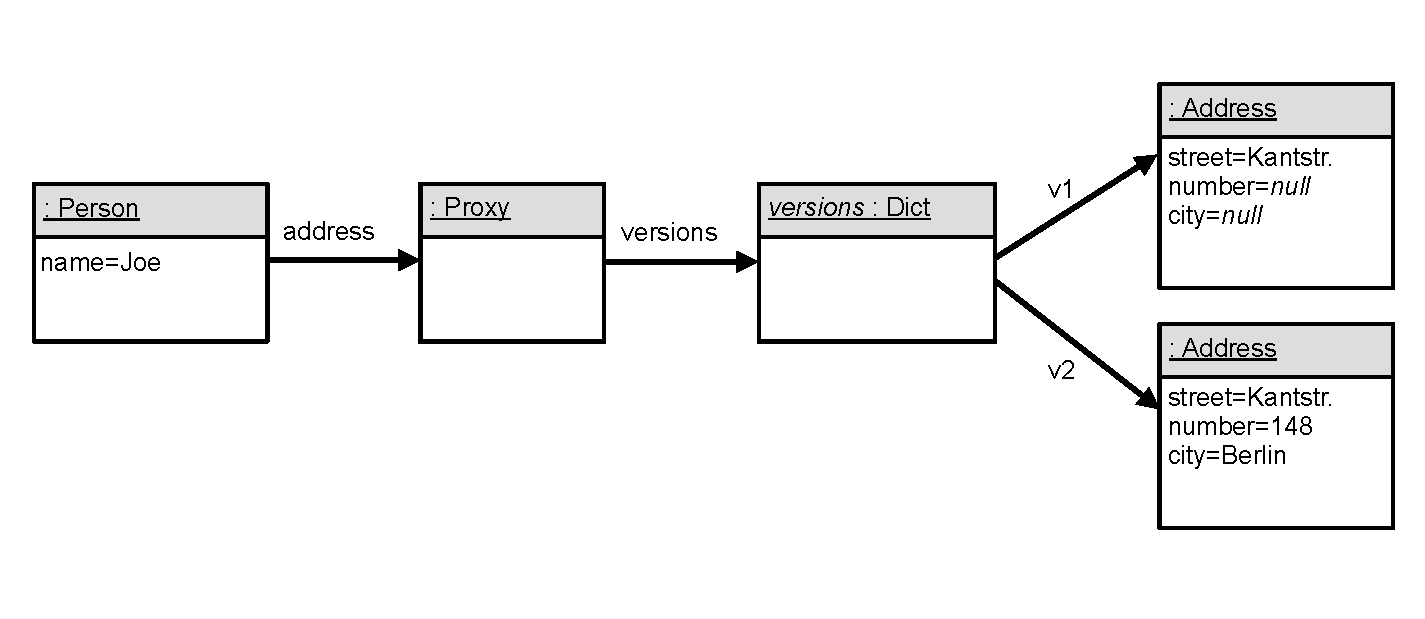
\includegraphics[width=\columnwidth]{figures/4_approach/7_proxyBasedVersionAwareReference.pdf}
    \caption{Using a proxy as version-aware reference to connect a \lstinline{person} object to two versions of an \lstinline{address} object.}
    \label{fig:ProxyBasedVersionAwareReference}
\end{figure}

The proxies fulfill three responsibilities:
\begin{enumerate}
    \item They know which versions are available for a particular object.
    \item They choose a particular version among all available dynamically using context information.
    \item They forward all interactions transparently to a chosen version.
\end{enumerate}

As mentioned in \autoref{sec:versions-system}, we use a source transformation to interpose proxies consistently between all mutable objects.
Our transformation wraps object literals and constructor functions into proxies, so all expressions that create new objects transparently return proxies.
The reference to the initial version of an object is only available to the proxy; the reference to the proxy is passed around instead.
Consequently, all references that would usually point to the same object point to the same proxy.
This way, proxies provide object identity.
Checks that would usually compare an object to another object now compare a proxy to another proxy.

Although keeping many versions around might put more pressure on the garbage collector, no special care has to be taken to release versions that are no longer required.
All object versions are referenced through a single proxy, so the versions get garbage collected with the proxy when it is no longer reachable.
So if you consider the \lstinline{Company} from \ref{fig:ObjectGraphWithReferencesResolvedAlongVersion2}, once you delete \emph{v1} of the \lstinline{ceo} reference, both \emph{v1} and \emph{v2} of the address object are collected.

The current version identifier of the system is accessible to the proxies.
The proxies forward to the same version of the object as long as the identifier remains constant.

\emph{To re-establish the previous version}, the version identifier is set to its predecessor.

\emph{To preserve the current version}, the version identifier is set to a new version.
The proxies forward interactions to other object versions or, when no such version of the object exist, create new versions.
Note that new versions are only necessary when a proxy is about to delegate manipulations.
As long as the state of an object is only read, the proxy reports values from a previous version as the old version of the object still reflects the current state.
To create a new version, a proxy copies the most recent previous version of the object.

Such a situation is shown in \autoref{fig:NewVersion}.
In a new version \emph{v3} of the system the proxy intercepts a manipulation, but has no object version it can forward to.
It therefore copies the most recent version of the object and forwards to the copy.

\begin{figure}[h]
    \centering
    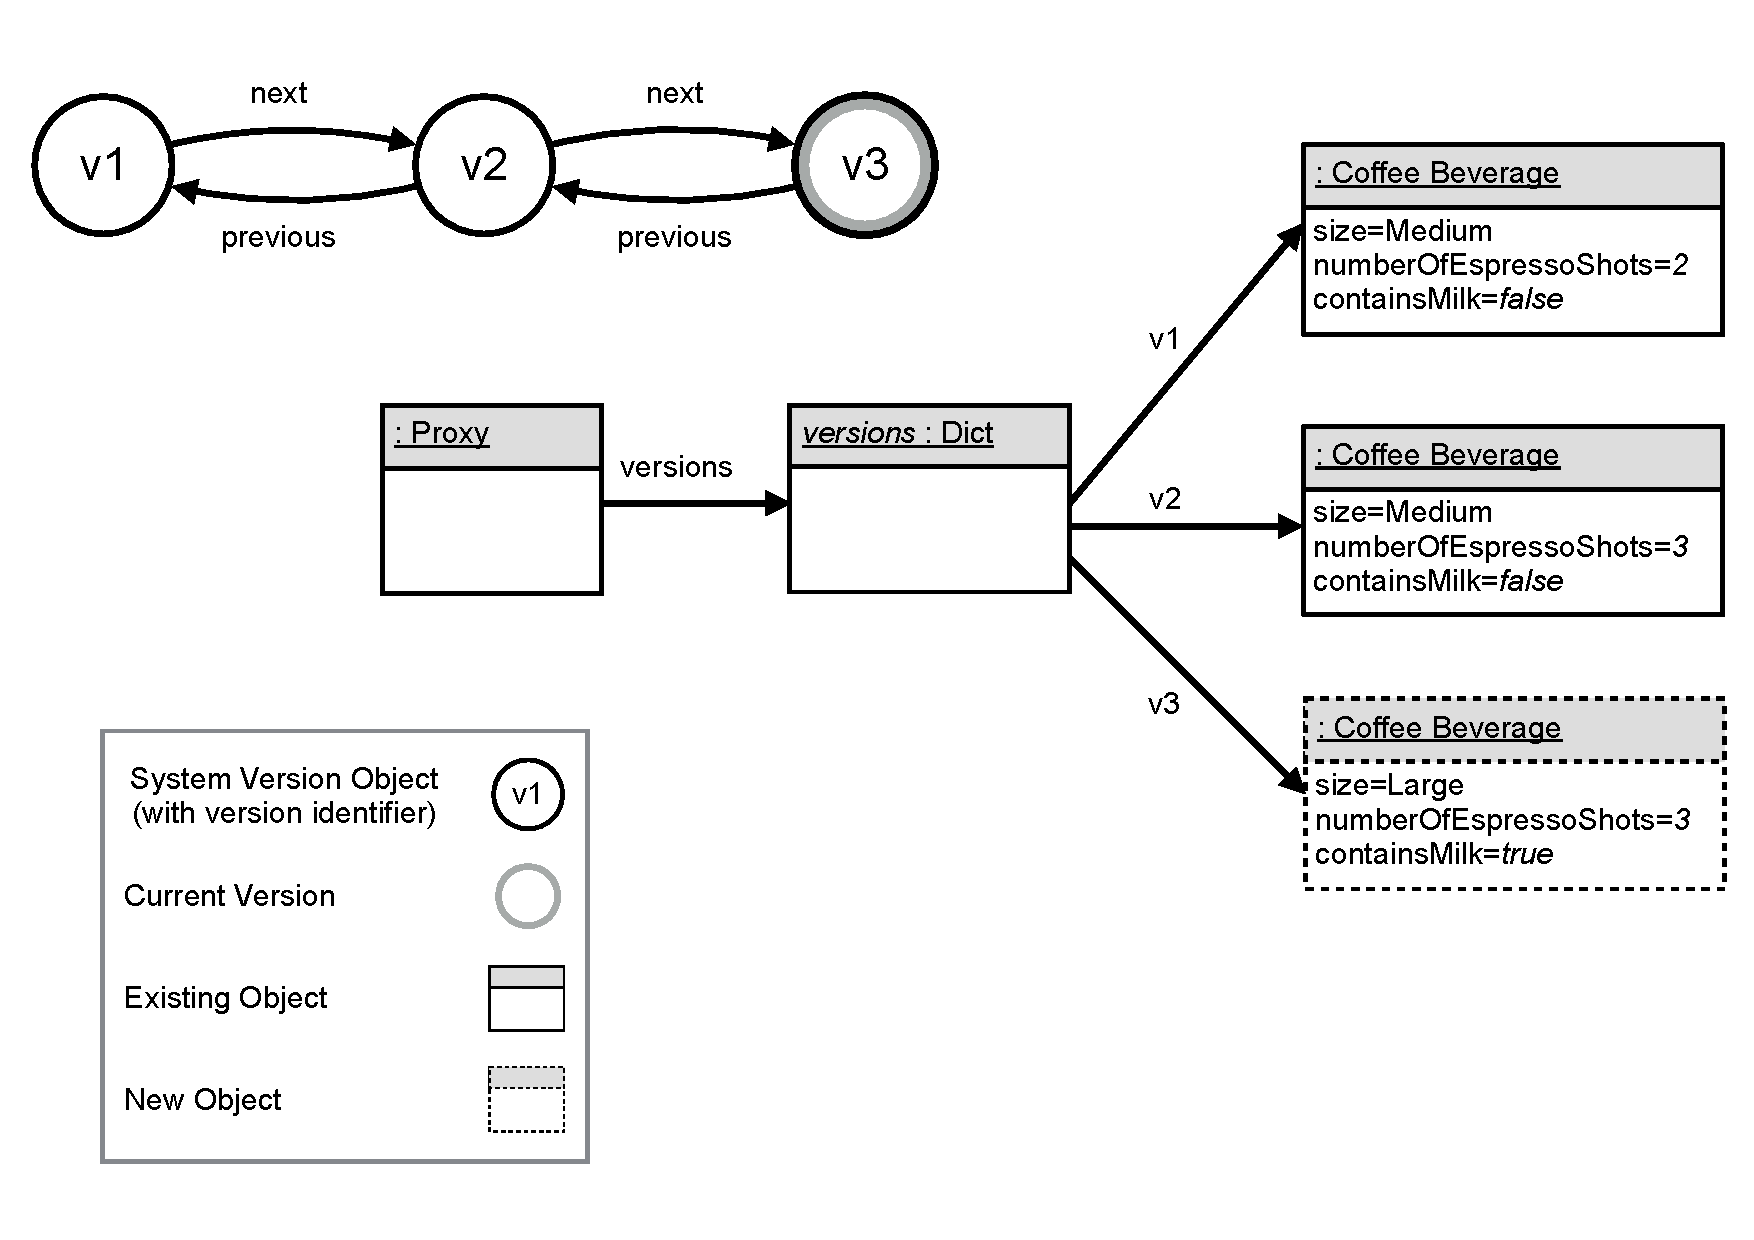
\includegraphics[width=0.86\columnwidth]{figures/4_approach/10_newVersionOfAnObject.pdf}
    \caption{A new version of an object is created for a new version of the system.}
    \label{fig:NewVersion}
\end{figure}

\paragraph{Limitations}

The current design allows to preserve and re-establish versions of the system.
Without further components, however, these versions only exist in memory and are not stored to disk.

Our current design does not support multiple predecessors or successors.

Another limitation of the current design is that the state of previous versions can be changed.
New versions of objects are not affected by changes to previous versions, but changes to object versions that have not been copied shine through in subsequent versions of the system.

In the future, the versioning might allow for branches and merging.
Changes to previous states could then be handled in branches that programmers may or may not merge into future versions.


 % content/5_implementation.tex
\section{Implementation} \label{chapter:IMPLEMENTATION}

This chapter describes our implementation of object-versioning using ECMAScript 6 proxies\footnote{\url{http://wiki.ecmascript.org/doku.php?id=harmony:direct_proxies}, accessed February 3rd, 2014} in the Lively Kernel.
At the time of this writing, these proxies only have draft implementations, and the JavaScript engines used by Chrome and Firefox provide differing preliminary implementations of their \ac{api}.
We use the \emph{harmony-reflect} library\footnote{\url{http://github.com/tvcutsem/harmony-reflect}, accessed February 3, 2014, used version 0.0.11} to abstract from these differences.

This chapter also presents our source transformation to insert proxies for ordinary references.
We use the \emph{UglifyJS}\footnote{\url{http://github.com/mishoo/UglifyJS2}, accessed March 12, 2014} library to implement source transformations.
UglifyJS parses without relying on JavaScript exceptions, so the transformation does not yield exceptions that could be caught by an open debugger.
In addition, UglifyJS supports Source Maps\footnote{\url{https://docs.google.com/document/d/1U1RGAehQwRypUTovF1KRlpiOFze0b-_2gc6fAH0KY0k/edit\#heading=h.ue4jskhddao6}, accessed May 2, 2014}, which allow the browser's developer tools to present the original sources during debugging.

\subsection{Using ECMAScript 6 Proxies for Object Versioning} \label{subsec:IMPLEMENTATION:1.2}

The ECMAScript 6 proxies \emph{stand in} for their target objects and intercept different interactions using \emph{traps}.
The implementation of the traps is provided by a separate \emph{handler} object.
When a proxy's handler does not implement a trap, the proxy forwards the intercepted interaction to the target.
On the hand, if all traps are implemented, all interaction can be handled without forwarding to the target object.

In our implementation, proxies delegate to one of multiple versions of an object.
In \autoref{fig:VersioningProxy} a proxy stands in for two versions of an \lstinline{address} object: The proxy's handler holds a reference to a \lstinline{versions} object, which in turn refers to the versions of the \lstinline{address} object.
The proxy's target is ommited from \autoref{fig:VersioningProxy} as we used the proxies as purely virtual objects.

\begin{figure}[h]
    \centering
    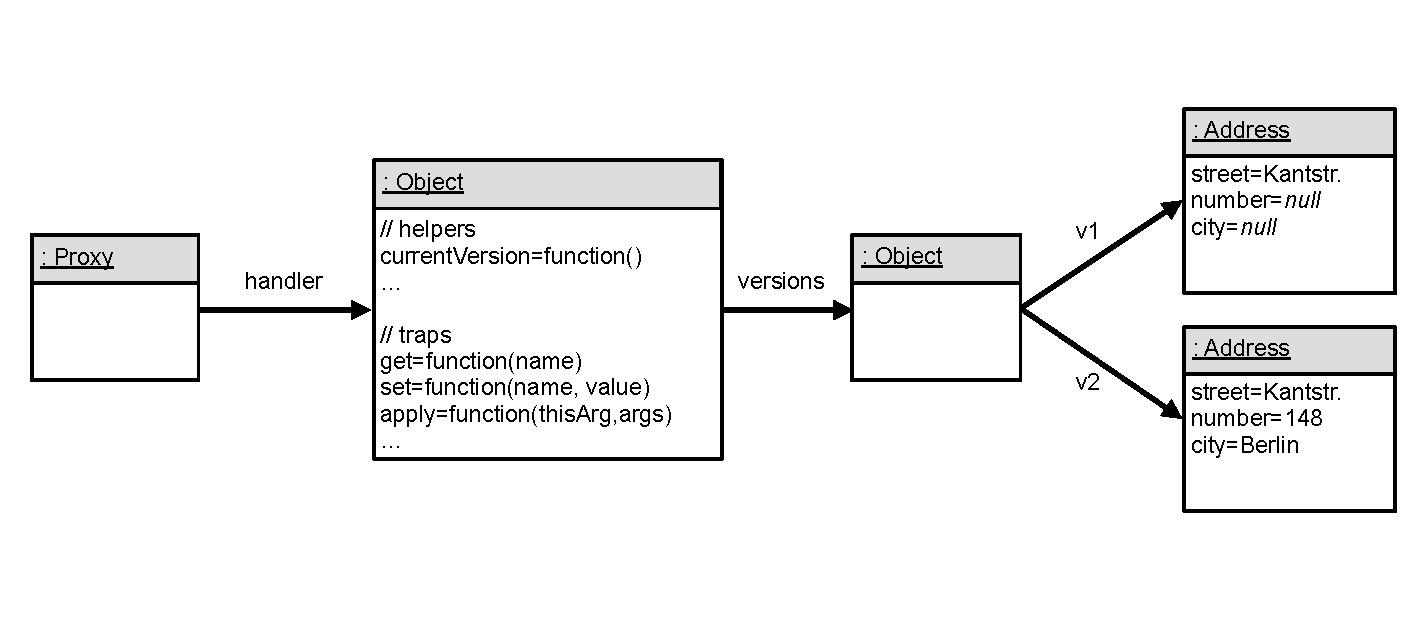
\includegraphics[width=\columnwidth]{figures/5_implementation/2_versioningProxy.pdf}
    \caption{A proxy with a handler that forwards to two versions of an \lstinline{address} object.}
    \label{fig:VersioningProxy}
\end{figure}

Our handler uses all available traps to forward to the current version of an object.
Each trap retrieves the current version of the object using the \lstinline{currentVersion} function, which selects the object version based on the active system version information.
The version information is available globally as \lstinline{lively.CurrentVersion}, an ordinary JavaScript object with three properties: an \lstinline{ID}, a \lstinline{predecessor}, and a \lstinline{successor}.

\begin{code}
currentVersion: function() {
    var objectVersion, systemVersion = lively.CurrentVersion;

    while(!objectVersion && systemVersion) {
        objectVersion = this.versions[systemVersion.ID];
        systemVersion = systemVersion.predecessor;
    }    
    return objectVersion;
}
\end{code}

All traps that intercept read-only access select the version to forward to using the \lstinline{currentVersion} function.
However, traps that intercept changes instead ensure a version of the object exists for the current system version, because the past cannot be allowed to change.
If no current version exists, the latest available version is copied and added to the \lstinline{versions} dictionary.
The traps that act in this way are \lstinline{set}, \lstinline{defineProperty}, \lstinline{deleteProperty}, \lstinline{freeze}, \lstinline{seal}, \lstinline{preventExtensions}, and \lstinline{apply}.
The \lstinline{apply} trap is included in this list because certain array functions such as \lstinline{push} and \lstinline{pop} are mutating, so when they are applied, a current version must be created.

The current version remains unchanged as long as the global \lstinline{lively.CurrentVersion} remains constant.
Changing the global version is an \emph{undo}, \emph{redo}, or \emph{commit} depending on whether the version is set to a previous, following, or new version.
The system provides convenience functions for these actions.
Using a global version of the system is reasonable as JavaScript is executed single-threaded, so the global version cannot be changed by another script.

\paragraph{Scope of the Versioning} \label{subsubsec:IMPLEMENTATION:5.2.1}
Using proxies allows multiple versions of most JavaScript objects, but certain objects represent the elements of the browser's \ac{dom} cannot be versioned with our implementation.
\ac{dom} objects are referred to from the browser's internal \ac{dom} structure, which is external to the JavaScript runtime.
In the Lively Kernel, this does not represent a problem, because the state of the \ac{dom} can be derived from morphs.
Whenever the system version changes, we update the \ac{dom} from the current set of visible morphs.

\subsection{Accessing All Mutable JavaScript Objects Through Proxies}

To be able to re-establish the system state with our versioning, we change the return values of all expressions that create new objects, arrays, and functions.
All these are mutable in JavaScript and might have arbitrary properties added to them.
Instead of letting these expressions return references to the new objects, the expressions return references to proxies for the objects.

In JavaScript, there are three categories of expressions that create new objects and for each of these one or more source transformations are required:
\begin{itemize}
    \item literals, \eg\lstinline|{age: 12}|
    \item constructors, \eg\lstinline|new Person(12)|
    \item some built-ins, \eg\lstinline|Object.create(prototype, {age: 12})|
\end{itemize}

\subsubsection{Wrapping Literal Expressions}

\begin{sloppypar}
We use source transformations to wrap literal expressions into calls to a \lstinline{proxyFor} function.
The expression \lstinline|{age: 12}| becomes \lstinline|proxyFor({age: 12})|, \lstinline{[a, b]} becomes \lstinline{proxyFor([a, b])}, and so forth.
We use a global proxy table to ensure the same proxies are returned for the same objects.
This proxy table is a weak-key dictionary, which allows the garbage collector to reclaim the objects used as keys.
Using the same proxies for the same objects is essential for identity checks to work correctly, so \lstinline{proxyFor(obj) === proxyFor(obj)} is always true.  
\end{sloppypar}

Literal object expressions can be wrapped in this way, but some expressions such as function declarations, accessor functions, and built-in functions need to be handled differently.

\subsubsection{Wrapping Function Declarations}

A \emph{function declaration} is a function literal that creates a named function and makes it available by the name in the surrounding scope:
\begin{code}
function add(a, b) { return a + b }
\end{code}

In contrast, a \emph{function expression} creates a function that needs to be assigned to a variable to be accessible:
\begin{code}
var add = function add(a, b) { return a + b }
\end{code}

Function expressions can create anonymous and named functions.
The previous example creates a named function.
Omitting the function name after the \lstinline{function} keyword would create an anonymous function.
While an anonymous function is always a function expression, a named function is either a function expression or a function declaration, depending on where it is expressed.
A function declaration cannot be nested into other statements such as variable assignments.

\begin{sloppypar} 
When a function declaration is wrapped into a \lstinline{proxyFor} function call, it becomes a function expression, meaning that it is no longer available by name in its surrounding scope.
After wrapping function declarations, they are assigned to matching variable names:~
\lstinline|function div() {}| becomes \lstinline|var div = proxyFor(function div() {})|.
In addition, because function declarations get hoisted in JavaScript, transformed function declarations are moved to the beginning of the defining scope.
\end{sloppypar}

\subsubsection{Wrapping Accessor Functions}

Accessor functions are functions that are executed instead of property reads or writes.
The following example uses an accessor function to allow reading a \lstinline{person}'s \lstinline{age} property, and have it calculated on access.

\begin{code}
var person = {
    birthdate: new Date(1984,27,5),
    get age() {
        return ageToday(this.birthdate);
    }
}
\end{code}

Wrapping the accessor function into a call to \lstinline{proxyFor} would not yield valid JavaScript syntax.
For this reason, the object is first created without the accessor function and the function is added afterwards using \lstinline{Object.defineProperty}.
The object literal and the call to \lstinline{Object.defineProperty} are wrapped into an anonymous functions that is immediately called to avoid polluting the variable bindings of the originally surrounding scope:

\begin{code}
var person = function() {
    var newObject = lively.proxyFor({
        birthdate: new Date(1984,27,5);
    });
    Object.defineProperty(newObject, "age", {
        get: lively.proxyFor(function age() {
            return ageToday(this.birthdate);
        })
        enumerable: true,
        configurable: true
    });
    return newObject;
}();
\end{code}

\subsubsection{Wrapping Constructor Functions} 

In JavaScript, all functions can be used as constructors when called with the \lstinline{new} operator and if so used, they need to return proxies.
We use the \lstinline{construct} trap to simulate the object construction and return a proxy around the newly created object.
This trap retrieves the current version of the constructor (Line~2), creates a new object with the correct prototype (Lines~3--4), calls the constructor with the new object as argument (Line~5), and returns a proxy for return value of the constructor function or, if the constructor returned a falsy value, the new object (Line~6).
\begin{code}
construct: function(dummyTarget, args) {
    var constructor = this.currentVersion(),
        prototype = constructor.prototype || {},
        newObject = Object.create(prototype),
        result = constructor.apply(newObject, args);
    return proxyFor(result || newObject);
}
\end{code}

\subsubsection{Wrapping Built-in Globals}

Some built-in global functions can be used to create new objects, such as the built-in constructors \lstinline{Object} and \lstinline{Array}.
Other globally accessible functions that create new objects include, for example, \lstinline{Object.create} and \lstinline{eval}.

We transform the built-in constructor functions by wrapping each global reference into calls to the \lstinline{proxyFor} function.
For example:
\begin{code}
new Object()  # => new proxyFor(Object)()
Object()  # => proxyFor(Object)()
Object.create()  # => proxyFor(Object).create()
\end{code}

The global symbols that are in this way: \lstinline{Array}, \lstinline{Boolean}, \lstinline{Date}, \lstinline{Function}, \lstinline{Iterator}, \lstinline{Number}, \lstinline{Object}, \lstinline{RegExp}, \lstinline{String}, \lstinline{JSON}, \lstinline{Math}, \lstinline{Intl}, \lstinline{XMLHttpRequest}, \lstinline{Worker}, \lstinline{XMLSerializer}, \lstinline{window}, and \lstinline{document}.

When a global function object is used as a constructor (line 1), the \lstinline{construct} trap returns proxies for the new objects as explained previously.
When they are used just as functions as in line 2 above, the \lstinline{apply} trap ensures that they return proxies.
When a property is read from a proxied object, as in line 3, the \lstinline{get} trap ensures the result is a proxy, and that when calling it, the proxy's \lstinline{construct} trap is triggered.
These transformations ensure that all functions of the globals return proxies.

\subsubsection{Wrapping \lstinline{eval}}

The \lstinline{eval} function is handled differently, because not only its result must be proxied, but also all objects created during the evaluation.
We ensure this by transforming the string argument to \lstinline{eval} before it is evaluated.
Alternatively, we could have overwritten the built-in functions to return proxies for new objects.
However, this alternative was rejected, because our implementation is a pure JavaScript library and makes itself use of the built-in types, so we would have to ensure that the original functions are still accessible to us.
Furthermore, some JavaScript engines do not allow overwriting all built-in globals and we want our implementation of object versioning to work in every JavaScript engine that supports the ECMAScript 6 proxies.

\subsection{Current Limitations of our Approach} \label{sec:IMPLEMENTATION:4}

Certain workarounds are required due to the preliminary implementation of ECMAScript 6 proxies in the JavaScript engines.
First, the proxies implement consistency invariants that compare return values of the traps to the state of the target.
Second, the proxies do not intercept the \lstinline{instanceof} operator, but always delegate to the current target.
Third, certain built-in JavaScript functions do not handle proxies correctly.
Finally, proxy traps appear in developer tools and thus impede debugging
These workarounds might no longer be necessary once the ECMAScript 6 specification gets released and fully implemented by the JavaScript engines.

\paragraph{Disabling Target Object Invariants}
All proxies require a target object and they are designed to ensure invariants between the return values of traps and the target's state~\cite{Cutsem2013TRP}.
For example, when an object's properties are made immutable through the \lstinline{Object.freeze} function, invariants ensure that the target object has in fact been frozen, even if the trap delegates the operation to another object.
As a result, freezing any version of an object would effectively freeze all versions.
As a workaround, we adapted our copy of the \emph{harmony-reflect} library to disable these consistency checks entirely.

\paragraph{Forwarding the \lstinline{instanceof} Operator}
The \lstinline{instanceof} operator can be used to test whether an object's prototype is in another object's prototype chain.
Since prototype of an object is a property and can be changed at runtime, it can be different in different object versions.
We provide a custom \lstinline{Object.instanceof} function, which implements the semantics of the \lstinline{instanceof} operator but delegates to object versions when applied with a proxy as argument.
All usages of the \lstinline{instanceof} operator are transformed into calls to \lstinline{Object.instanceof}.

\paragraph{Unwrapping Versions for Native Code} \label{subsec:IMPLEMENTATION:4.3}
Some built-in JavaScript functions do not work correctly with proxies, react with errors, return wrong results, or silently ignore calls when applied with proxies as arguments.
These built-in functions include, for example, the \lstinline{concat} function of array instances, all functions that manipulate the browser's \ac{dom}, string instance methods that take \lstinline{RegExp} arguments, and the \lstinline{onreadystatechanged} property of \lstinline{XMLHttpRequest} objects.
These problematic functions need to be provided with actual objects instead of proxies.
Our apply trap special cases problematic built-in functions and unwraps proxies as needed.

\paragraph{Proxies Impede Developer Tools}
The current ECMAScript 6 proxies are partly implemented in JavaScript and every trapped object interaction is visible in multiple frames in the debugger.
Consequently, the stack of the debugger is cluttered with frames that belong to the proxy implementation, not to application code.
Moreover, the developer tools do not handle proxies correctly under all circumstances, show the wrong inspect strings, or always step over proxied functions.
We currently have no workaround for these issues.


 % content/6_evaluation.tex
\section{Evaluation} \label{chapter:EVALUATION}

The presented approach has been evaluated concerning functionality and
practicability in two different ways. \emph{First}, we used the
\emph{Octane} benchmark
suite\footnote{\url{http://code.google.com/p/octane-benchmark/},
  accessed February 3, 2014, at version 26} to evaluate the behavior
and performance of our implementation. Octane is one of the standard
benchmark suites for JavaScript \acp{vm}.

\emph{Second}, we checked our implementation with the Lively Kernel. We
implemented the versioning as a base layer of Lively Kernel in order
to have object versioning enabled for the entire system
eventually. The most recent commit of Lively we used for the
evaluation is
\emph{ed0586d80}\footnote{\url{http://github.com/LivelyKernel/LivelyKernel/commits/ed0586d80},
  accessed May 9, 2014}. In this version, most of the Lively Kernel's
code passed the transformations.  Only the Lively Kernel's bootstrap
code, its module system, extensions to built-in types, and our
implementation itself are excluded from the source transformations.
All modules loaded after these parts are transformed at load-time to
enable versioning for them. 

We have gained various insights by making the concepts run for a large
JavaScript application such as the Lively Kernel. The Lively Kernel
makes use of many features of the JavaScript language and the browser
environment such as built-in objects and functions. These are not part
of the ECMAScript standard, but are nevertheless used by many
applications. For example, the browser offers functions to manipulate
its \ac{dom}, which the Lively Kernel uses for rendering. These
built-ins are not covered by Octane or other popular JavaScript
benchmark suites.

\paragraph{Machine Configuration}
All tests and measurements were done on May 9, 2014 using a Macbook
Air with a 2 GHz Intel Core i7 and 8 GB main memory, Mac OS X 10.9.2,
and version 34.0.1847.131 of Chrome.  All presented measurement
results were averaged over five runs. We used Chrome for all
experiments because Lively currently works best in Chrome.

\subsection{Functionality of Version-aware References} \label{sec:EVALUATION:2}

\subsubsection{Testing with Octane}

\paragraph{Method}
We transformed the Octane benchmarks with our source transformations,
executed the resulting code, and then checked for JavaScript errors
and compared the results of the transformed benchmarks to their usual
results. We did this to test two aspects.  First, to test whether our
source transformations yield syntactically correct JavaScript code for
the benchmarks.  Second, to test whether our proxy-based version-aware
references, inserted by the source transformations, allow to run the
benchmarks without errors and with the expected results.

\paragraph{Results}
All benchmarks in this suite run without errors and return the same
results as if executed without any source transformations.  Therefore,
at least for these tests, our source transformations produce working
source code and our proxy-based version-aware references forward
correctly to object versions. During the development of our system,
the \emph{DeltaBlue} benchmark revealed a problem when proxies are
used as prototypes of objects.  We reported the issue to the
\emph{harmony-reflect}
repository\footnote{\url{http://github.com/tvcutsem/harmony-reflect/issues/18},
  accessed April 23, 2014}.  The problem was identified as an issue
with the \emph{v8} JavaScript
engine\footnote{\url{http://code.google.com/p/v8/issues/detail?id=2804},
  accessed April 23, 2014}.  We implemented a workaround for this
problem, but the issue was subsequently fixed, rendering the
workaround redundant.

\paragraph{Discussion}
The proxies behave correctly like particular versions of objects in
the situations tested by the benchmarks.  While these benchmarks do
not test JavaScript's features systematically, they cover a wide range
of important language features.

\subsubsection{Testing with the Lively Kernel}

\paragraph{Method}
We transformed the JavaScript modules of the Lively Kernel at
load-time to test whether it loads and works correctly with our
proxy-based version-aware references.  Furthermore, we tested whether
the system allows re-establishing versions of the Lively Kernel's
state in practice.  Here, we tried multiple example scenarios,
including the undo of changes to the state and behavior of basic
morphs, morph compositions, and the state of more complicated
graphical applications such as text editors and developer tools.  With
this, we tested that the source transformations yield valid JavaScript
code for the modules of the Lively Kernel, that the version-aware
references delegate to the correct versions of objects, and that the
version-aware references are used consistently.

\paragraph{Results}
The Lively Kernel loads when its modules are transformed to use our
version-aware references.  Most of its basic functionality works as
expected and we were able to preserve and re-establish runtime states
of multiple examples.  However, not all functionality works as
expected and we were, thus, not able to re-establish all preserved
states.  In particular, we learned about the many built-in functions
that currently do not handle proxies correctly in Chrome and for which
we implemented the workaround described in
Section~\ref{subsec:IMPLEMENTATION:4.3}.

\paragraph{Discussion}
Most of the tested functionality of the the Lively Kernel works
correctly.  This includes the entire bootstrap process, rendering
graphical objects, loading parts from the Lively Kernel's Parts Bin,
and using the Lively Kernel's halo controls.  However, certain
functionality of the Lively Kernel is not yet working correctly or
even yields errors.  The remaining issues here are expected to be
problems related to the built-in functions that do not work correctly
when proxies are provided as arguments.  Our implementation already
unwraps object versions from proxies for many built-in functions, as
explained in Section~\ref{subsec:IMPLEMENTATION:4.3}, but the
configuration does not cover all problematic built-in functions yet.

At the same time, the proxies are not yet fully supported by Chrome
and we expect these issues not to be problematic anymore when proxies
get fully implemented by Chrome's JavaScript engine.

\subsection{Practicability: Memory Consumption} \label{sec:EVALUATION:3}

We measured the memory overhead imposed by the version-aware
references and how much memory is consumed when versions of the Lively
Kernel's state are preserved. Therefore, we used Chrome's built-in
memory
profiler\footnote{\url{http://developers.google.com/chrome-developer-tools/docs/heap-profiling},
  accessed May 8, 2014}.  It allows to take heap snapshots.  These
snapshots contain all reachable JavaScript objects.  For each
snapshot, Chrome shows the total size in MB.

\subsubsection{Memory Overhead of Version-aware References}

\paragraph{Method}
We measured the memory required for loading a Lively Kernel world with
and without version-aware references.  We took heap snapshots right
after the world was completely loaded without interacting with the
system.  We used an empty Lively Kernel world for this experiment and
did not preserve any versions.

\paragraph{Results}
As shown in Figure~\ref{fig:MemoryOverheadForReferences}, loading an
empty Lively Kernel world requires three times more space with proxies
than without proxies.

\begin{figure}[h!]
    \centering
    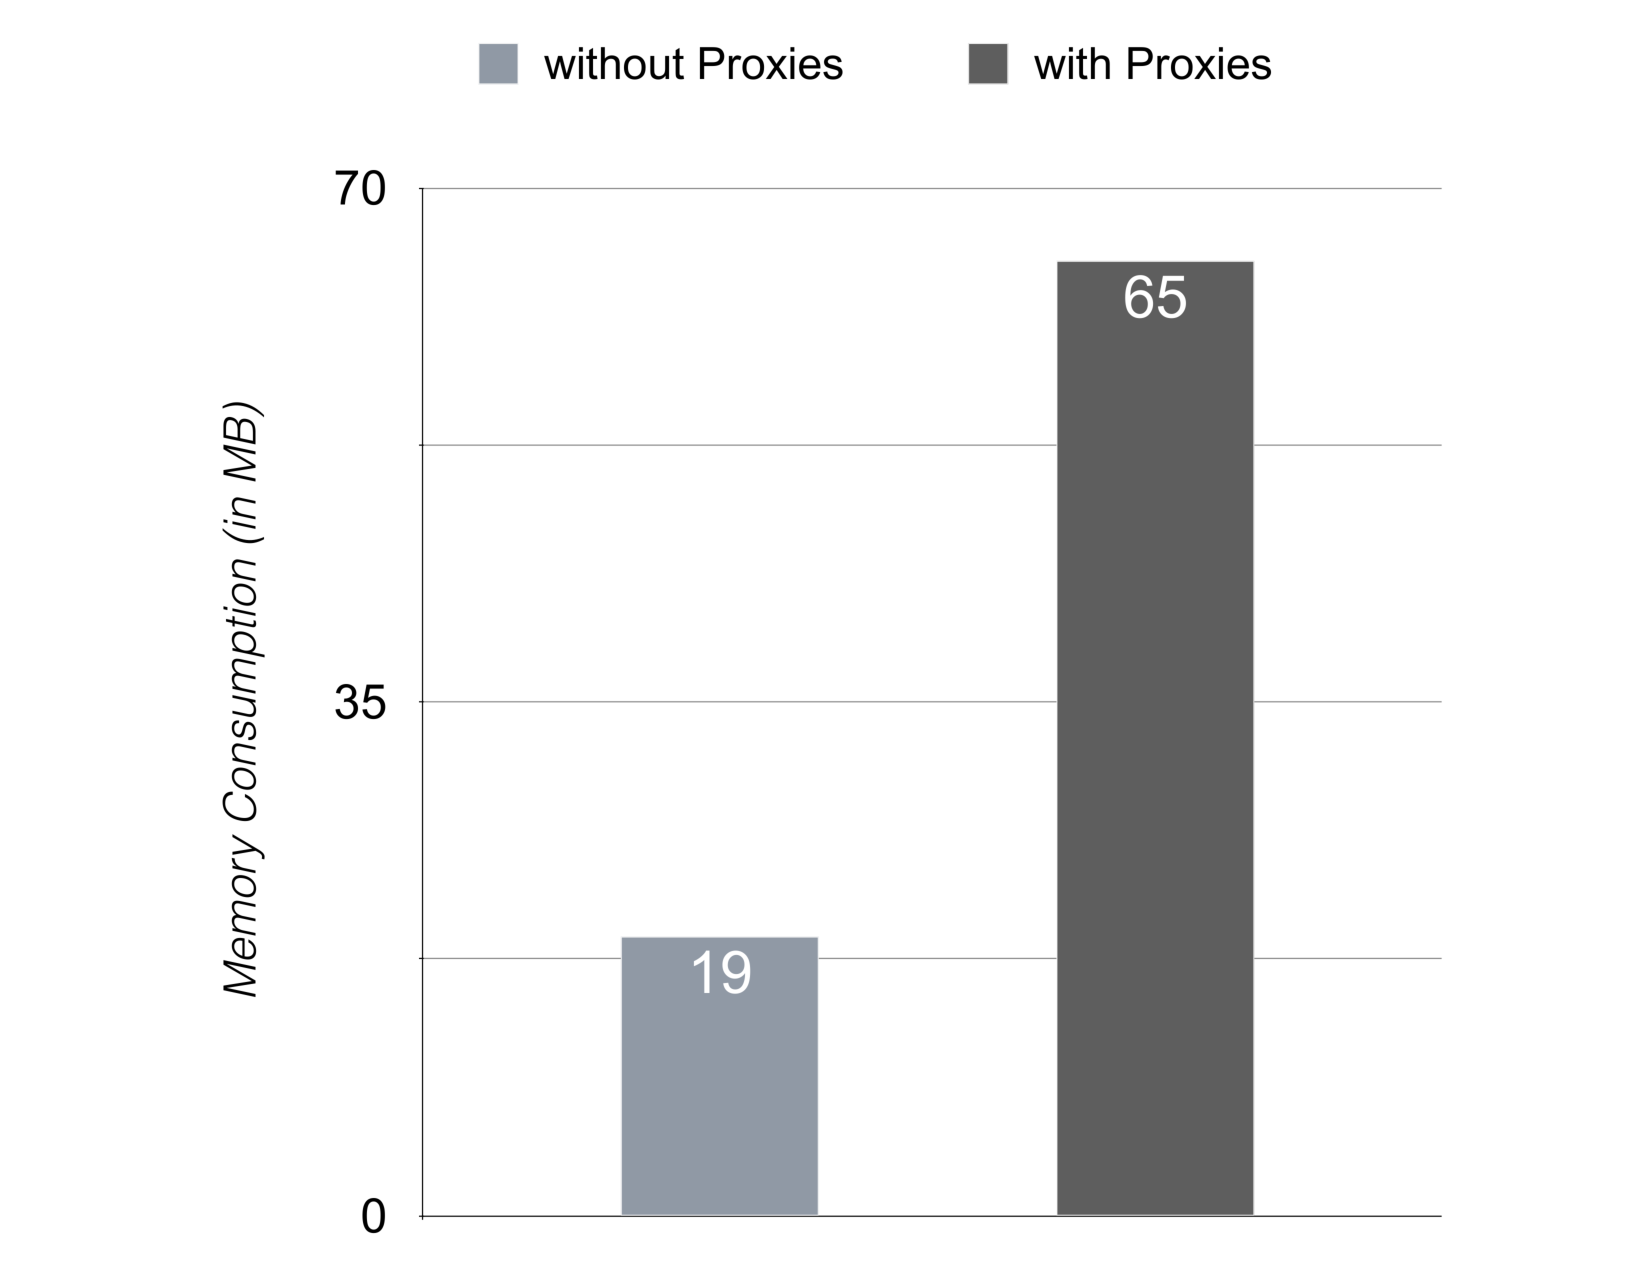
\includegraphics[width=0.7\columnwidth]{figures/6_evaluation/1_memoryOverhead.pdf}
    \caption{Memory consumption when starting a Lively Kernel world with and without proxies.}
    \label{fig:MemoryOverheadForReferences}
\end{figure}

\paragraph{Discussion}
When loaded with proxies, the system requires space for the proxies.
Even without preserving multiple versions of any object, the system
uses a proxy for each object.  These proxies require additional space:
Each proxy comprises of at least a proxy object, a proxy handler
object that specifies the proxy's behavior, and an object to hold all
object versions.

We expect the memory overhead to increase linearly with the number of
objects accessed through proxies.  While the system creates proxies
for most objects, it does not use proxies for all objects.  In
particular, it does not create proxies for objects that are present
before our implementation of object versioning is loaded and all
objects used by our implemenation itself.  We expect the number of
objects that are excluded from versioning to be relatively stable.
All additional objects created at runtime will be accompanied by
proxies. The memory overhead does not appear to be problematic at the
moment.

\subsubsection{Memory Consumption When Preserving Versions}

\paragraph{Method}
We measured how much memory is consumed when multiple versions of the
system are preserved while working on a group of morphs.  The three
states for which we took snapshots are shown as \circnum{1},
\circnum{2}, and \circnum{3} in the upper half of
Figure~\ref{fig:MemoryOverheadForVersions}.  In particular, we did the
following in this experiment:
\begin{enumerate}
\item Version 1: We measured the memory consumed at State \circnum{1}
  in the initial version of the system.
\item Version 2: We created a new version to preserve the initial
  state and then changed the state towards State \circnum{2} in the
  new version. Subsequentely, we measured the memory consumption for
  this state.
\item Version 3: We preserved the previous state, changed the state to
  State \circnum{3} in a third version, and measured the memory
  consumption again.
\end{enumerate}

This experiment does not show how much memory is required exactly for
storing multiple versions of particular objects.  Instead, the
experiment shows the overall memory consumption of the entire Lively
Kernel while our implementation is used realistically.

The snapshots include the size of all reachable JavaScript objects,
not just the versions of the morph objects shown
Figure~\ref{fig:MemoryOverheadForVersions}.  The reachable JavaScript
objects in these snapshots are all objects of the Lively Kernel.  For
example, the tools we used to change the morph states between the
snapshots are implemented in JavaScript.  Their state is part of the
system state.

We closed all tools before taking memory snapshots to exclude their
state from the snapshots, but the Lively Kernel caches some state of
these tools.  The cached state might be different in the three states.
Thus, the size of the cached state might be different in the three
snapshots.  Furthermore, previous versions of the cached state might
get preserved with the versions of the system.

\paragraph{Results}
Figure~\ref{fig:MemoryOverheadForVersions} shows the size of the three
snapshots.  State \circnum{1} required the least memory.  State
\circnum{2} requires 1.8 MB more memory.  It also requires 0.3 MB more
memory than State \circnum{3}.

\begin{figure}[h]
    \centering
    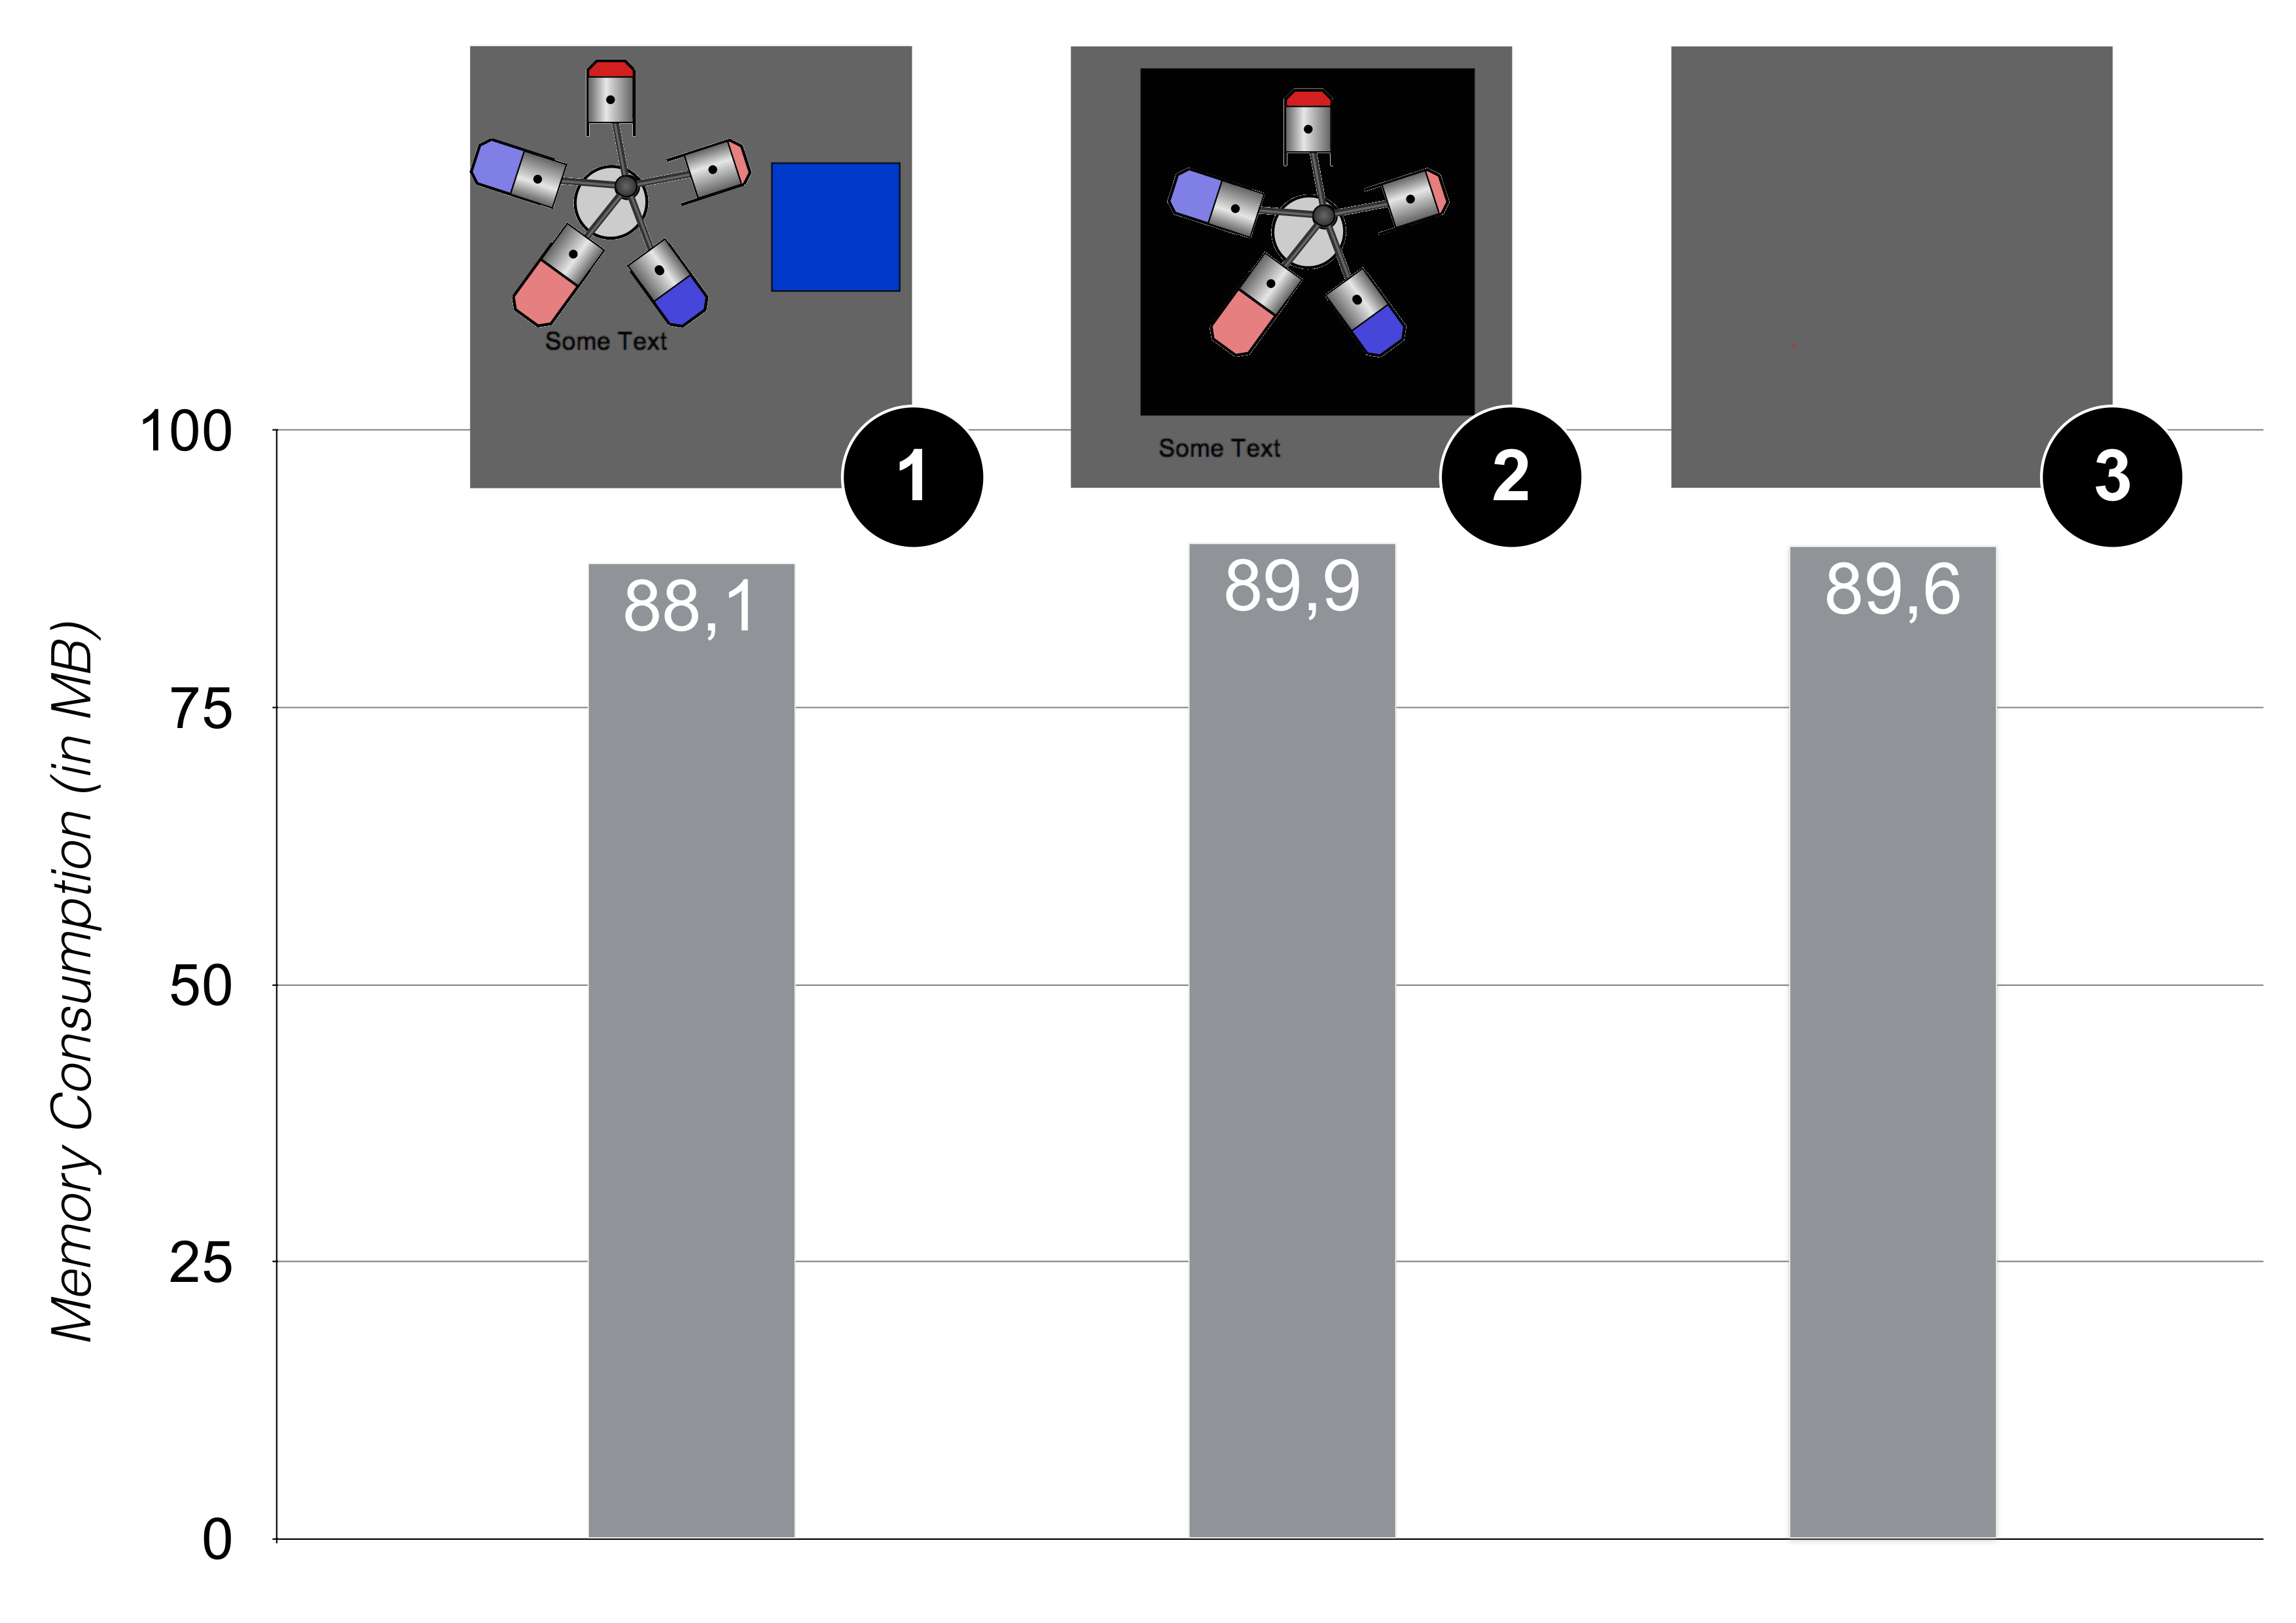
\includegraphics[width=0.76\columnwidth]{figures/6_evaluation/2_memoryForVersions.png}
    \caption{Memory consumed for three different states when the previous states are preserved in separate versions.}
    \label{fig:MemoryOverheadForVersions}
\end{figure}

\subsubsection{Discussion}

The sizes of the three snapshots are not significantly different.
Even though it is not clear how much space is used for preserving the
previous states of just the morphs, the results show that preserving
system states requires relatively little memory.  Our implementation
does not copy all objects for each version, but only creates copies
when objects change from one version to another, effectively storing
only the differences between system versions.  Therefore, the memory
required for preserving versions of the system depends on how objects
change in each version.  In the presented scenario, the space required
for preserving the three states is insignificant to the space already
required for running the Lively Kernel.

The results also show that the memory consumption does not always
increase even when previous states are preserved: State \circnum{3}
requires less memory than State \circnum{2}.  One explanation for this
is that not all objects are preserved with the versions.  One category
of such objects are the objects that only provide access to the
elements of the browser's \ac{dom}, as described in
Section~\ref{subsubsec:IMPLEMENTATION:5.2.1}.

\subsection{Practicability: Impact on Execution Speed} \label{sec:EVALUATION:4}

We measured the overhead that our implementation imposes on running
benchmarks and the Lively Kernel. A discussion of the results follows
at the end of this section.

\subsubsection{Octane Benchmark Suite}

\paragraph{Method}
We ran the Octane benchmarks\footnote{Note: We reduced the input size
  of the Splay benchmark by an order of magnitude to prevent the
  browser from prompting for user input during the benchmark's
  execution. The prompt is triggered due to the long time required to
  run the benchmark. It cannot be disabled and would influence the
  benchmark result.} with and without previous transformation of the
benchmark code and, therefore, with and without version-aware
references.  The source transformations for this were done separately
before measuring the execution times.

\paragraph{Results}
Figure~\ref{fig:ExecutionOverhead} shows how much more time the
benchmarks take when their source is transformed before execution and
references are, therefore, version-aware.  Executing individual
benchmarks takes between 90 and 405 times longer with version-aware
references than without.  On average the execution is slowed down by a
factor of 187.5.

\begin{figure}
  \centering
    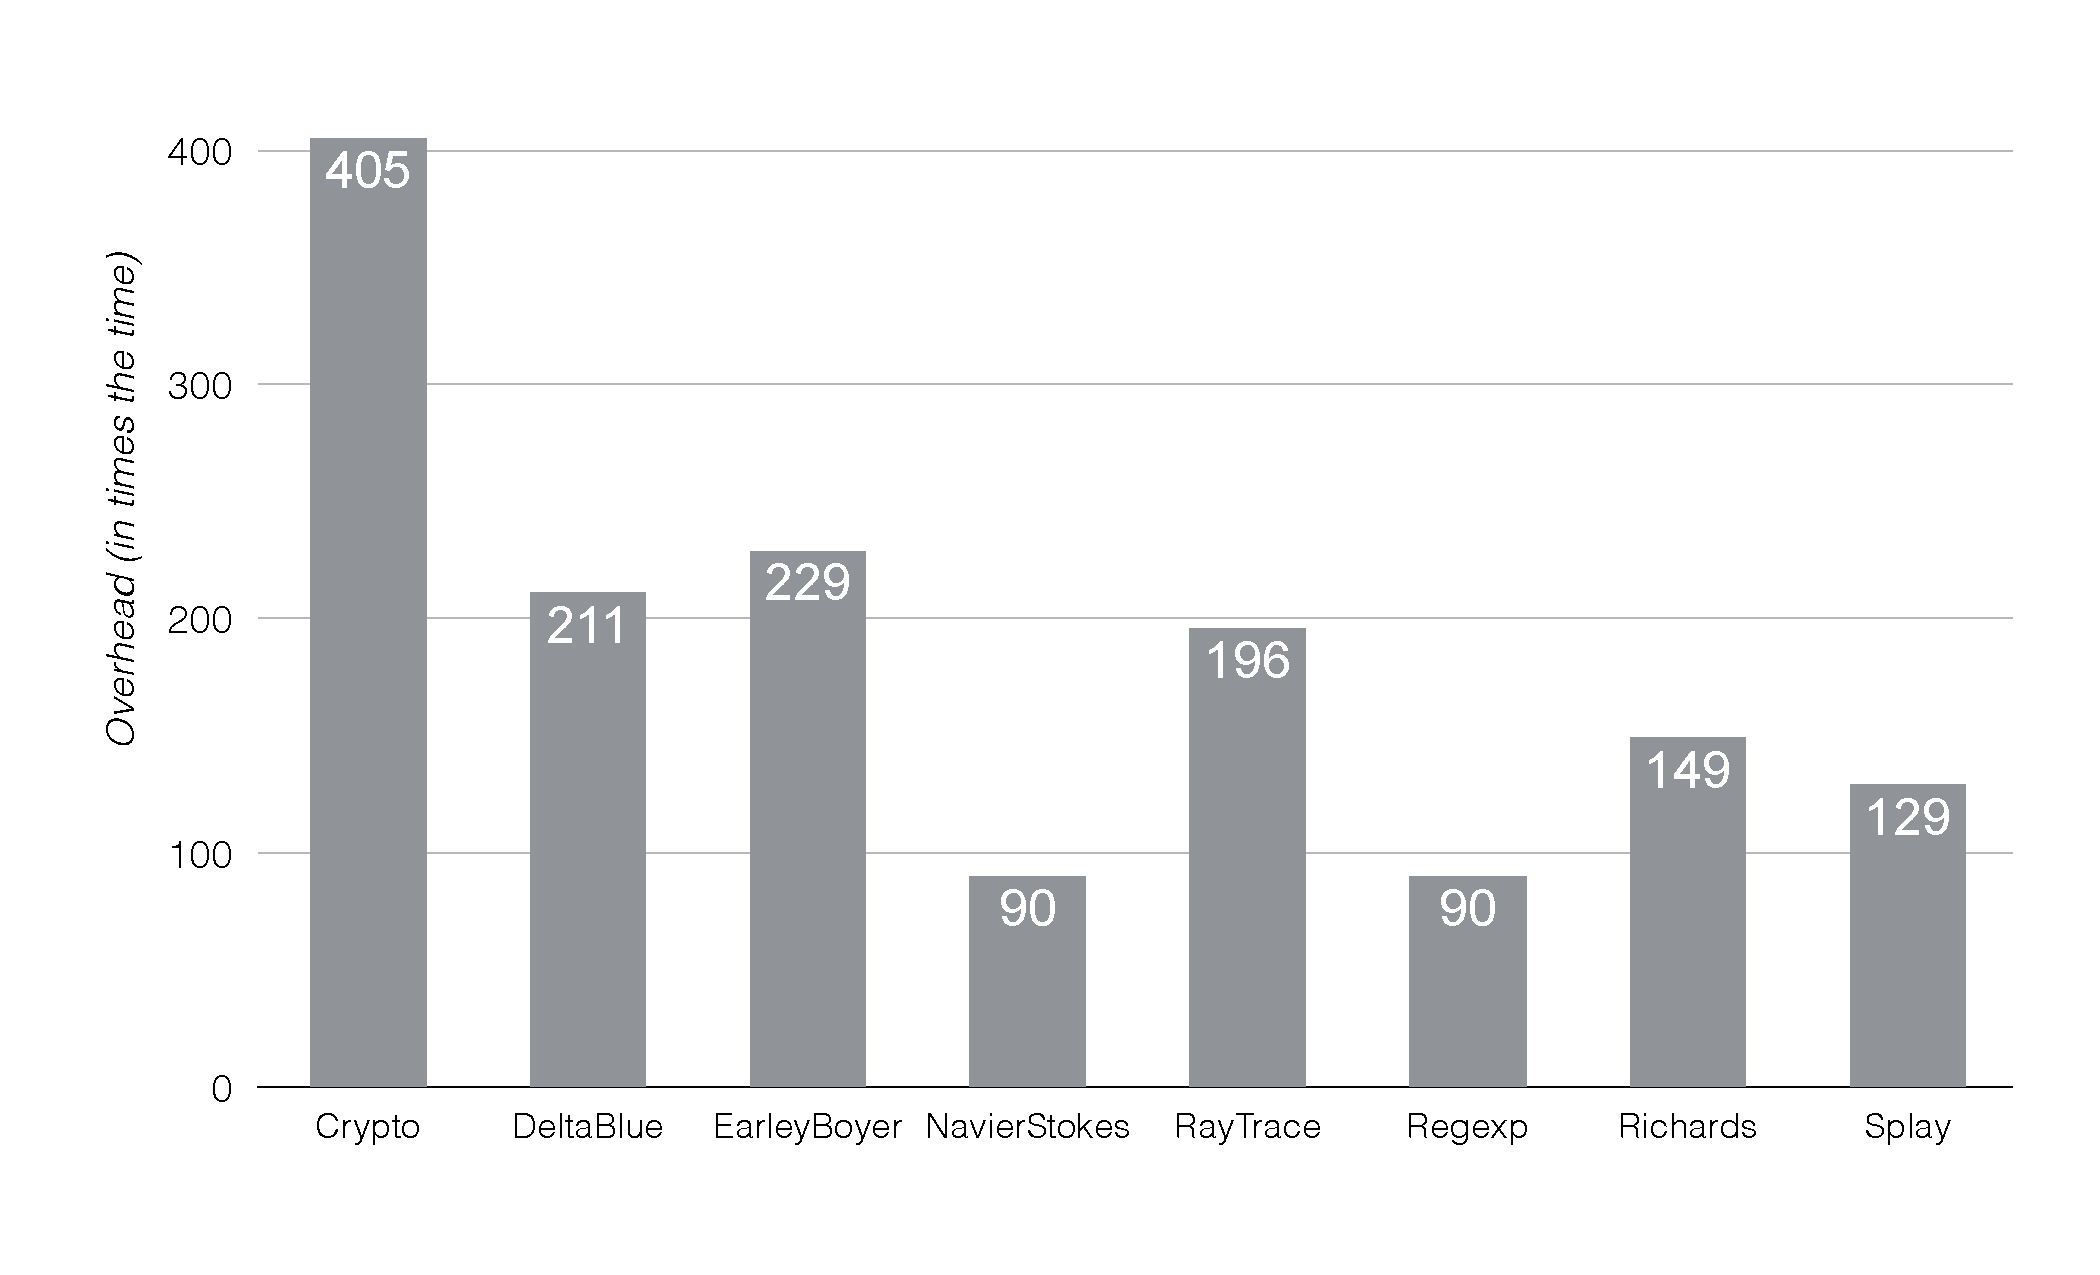
\includegraphics[width=\columnwidth]{figures/6_evaluation/3_executionOverhead.pdf}
    \caption{Execution overhead for the Octane benchmark suite.}
    \label{fig:ExecutionOverhead}
\end{figure}

\subsubsection{Microbenchmarks}

We implemented a microbenchmark to measure the overhead the proxies
impose on resolving references.  In particular, the microbenchmark
shows how much time the proxies require to intercept and forward
property reads to the single version of an object.

\paragraph{Method}
We measured how long it takes to resolve a reference as well as read
and call a function property a million times.  The reference connects
a \lstinline{client} object to a \lstinline{server} object, which has
an \lstinline{empty} function:

\begin{code}
for (var i=0; i < 1000000; i++) {
    client.server.empty();
} 
\end{code}

We compared the execution times of three different setups:

\begin{description}
\item[Setup 1] The \lstinline{client} object holds a reference
  directly to the \lstinline{server}.
    \item[Setup 2] The \lstinline{client} object holds a proxy as its
      \lstinline{server} property. In this setup, we used the proxy
      handler described in Section~\ref{subsec:IMPLEMENTATION:1.2} for
      the proxy. The proxy has access to the actual \lstinline{server}
      object as one of its version objects. It selects the
      \lstinline{server} object when it intercepts the property read.
    \item[Setup 3] The \lstinline{client} object's \lstinline{server}
      property is also a proxy but one created with a fixed target and
      without proxy handler. The fixed target is the
      \lstinline{server} object to which the proxy then forwards by
      default.
\end{description}

In all setups, the \lstinline{server} object holds a reference that
directly refers to the \lstinline{empty} function.

\paragraph{Results}
Table~\ref{table:microbenchmarkResults} shows the results of running
the microbenchmark in the three setups.  Using a proxy with our proxy
handler takes three orders of magnitude more time than using an
ordinary reference does: Instead of on average 10 milliseconds the
test requires on average about 11000 milliseconds to finish.  The
difference between \emph{Setup 3} and \emph{Setup 1} is an order of
magnitude less: 2000 milliseconds compared to 10 milliseconds.  This
shows that even a proxy with a fixed target and the default proxy
behavior slows down the execution of the microbenchmark close to 200
times.

\begin{table}[h]
\begin{center}
\begin{tabular}{| l | l |}
\hline
\emph{Setup 1} & 10 milliseconds \\ \hline
\emph{Setup 2} & 11000 milliseconds \\ \hline
\emph{Setup 3} & 2000 milliseconds \\ \hline
\end{tabular}
\end{center}
\caption[Table caption text]{Times to run the three setups of the microbenchmark.}
\label{table:microbenchmarkResults}
\end{table}

\subsubsection{Loading a Lively Kernel World}

\paragraph{Method}
We measured how long it takes to load a specific Lively Kernel world
with and without source transformations and, thus, proxies.  Loading a
world includes requesting the required modules from the Lively
Kernel's server, client-side code to resolve dependencies among those
modules, evaluating the code of the loaded modules, and deserializing
the graphical state of the world's scenegraph.  Additionally, in case
proxies should be used, the sources of all modules also are
transformed while loading the world.

\paragraph{Results}
It takes eight times more time to load a world with object versioning:
instead of around 4 seconds, the user would have to wait around 32
seconds until the world becomes responsive.

\subsubsection{Typical Lively Kernel Interactions}

\paragraph{Method}
We measured the time three user interactions take when using proxies
and compared this to the time the interactions usually take.  We
measured the time from the user events until the single-threaded
JavaScript engine becomes responsive again programmatically.  The
three typical interaction we chose to investigate are: bringing up the
halo buttons on a particular morph, opening the Lively Kernel's main
menu, and opening the Lively Kernel's System Code Browser.

We chose these three interactions as we expect them to be more
impacted by the version-aware references compared to interactions that
are more browser-supported and less reliant on the execution of
JavaScript code such as dragging elements around the screen.  All
three interaction trigger code from multiple different modules,
including event handling code, rendering code, and tool-specific code.

\begin{figure}[h!]
    \centering
    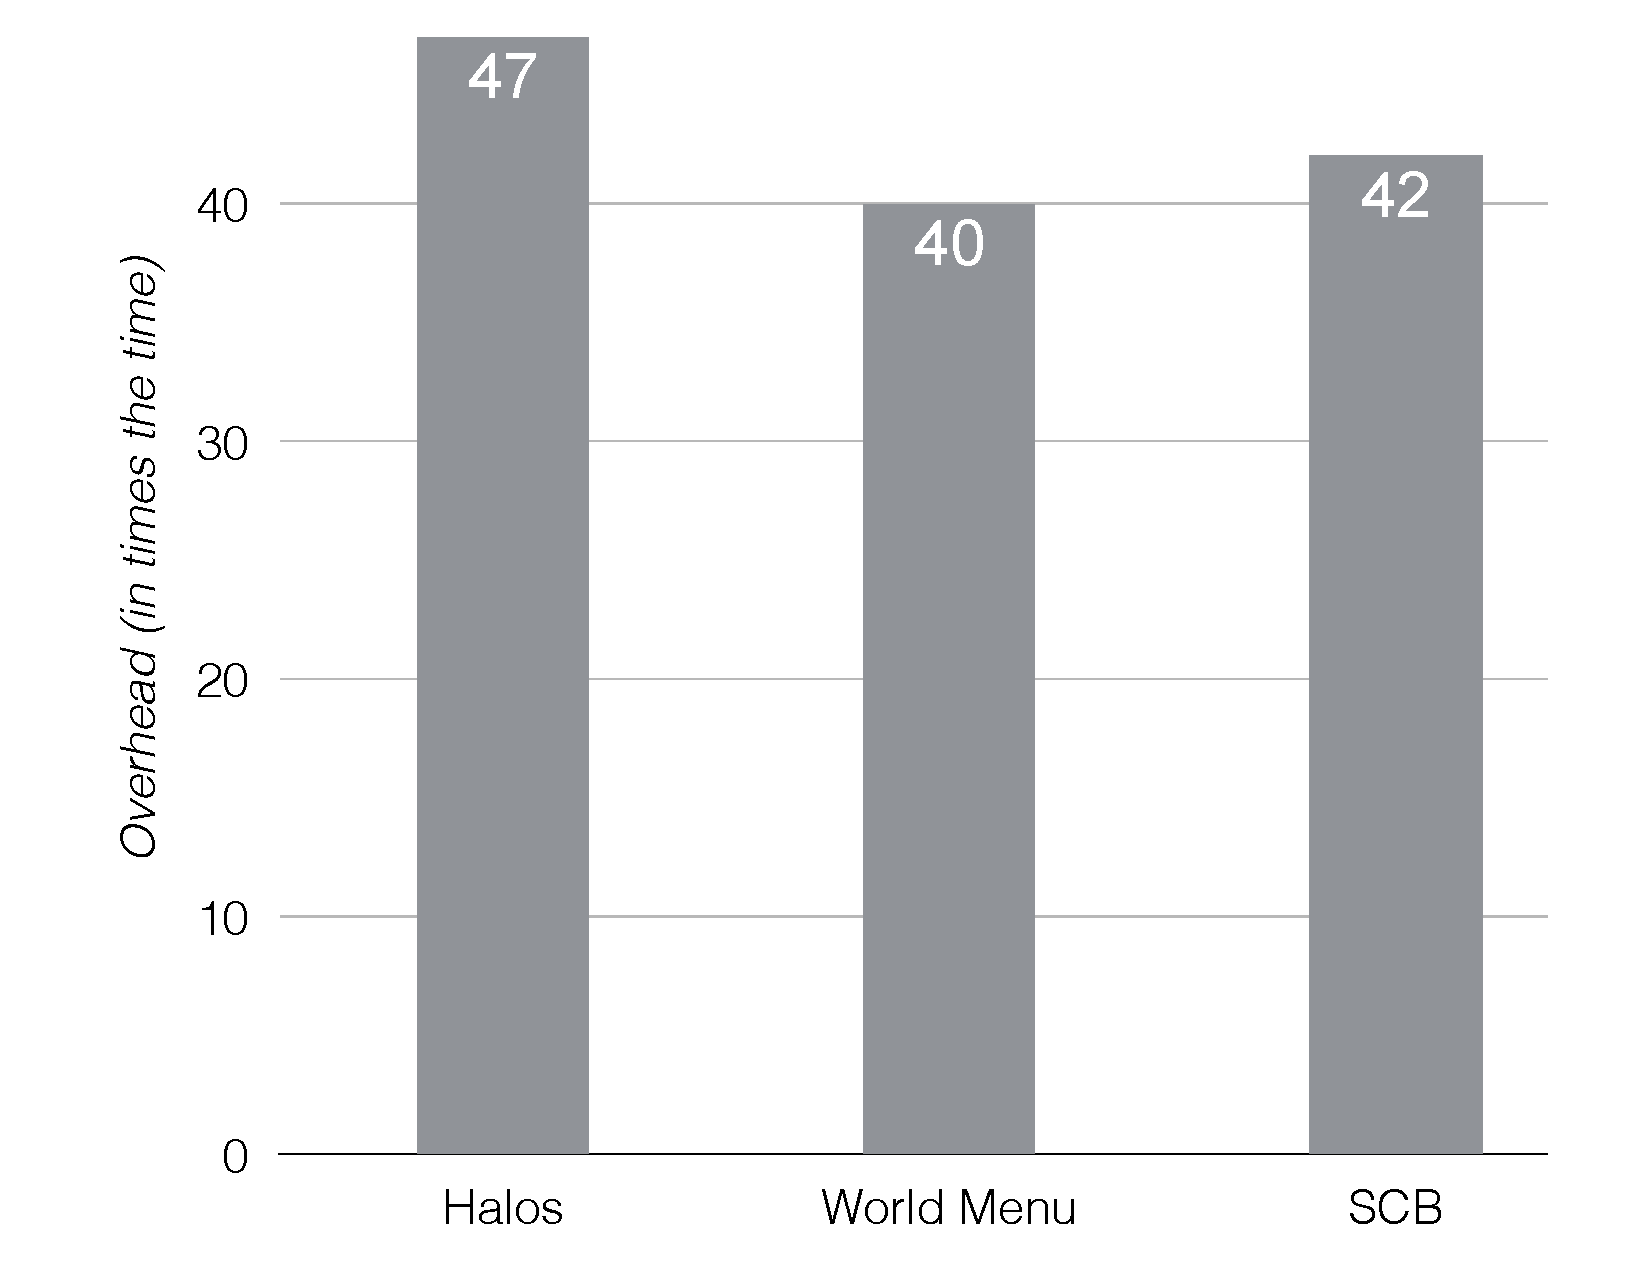
\includegraphics[width=0.64\columnwidth]{figures/6_evaluation/4_livelyInteractionsOverhead.pdf}
    \caption{Execution overhead for three user interactions in the Lively Kernel.}
    \label{fig:LivelyInteractionsOverhead}
\end{figure}

\paragraph{Results}
Figure~\ref{fig:LivelyInteractionsOverhead} shows the results.  Each
of the three interactions takes on average 43 times the time when
triggered after the system was loaded with proxies.

\subsubsection{Discussion of the Execution Overhead}

The results of our evaluation show that the execution overhead is
currently impractical.  The Octane benchmarks indicate that executing
real JavaScript programs takes two to three orders of magnitude more
time.  Similarly, the Lively Kernel tools are significantly less
responsive. Even though we expected a certain execution overhead with our
approach, the current overhead is too high.

The microbenchmarks show that a considerable part of the overhead is
introduced by using the ECMAScript 6 proxies.  Even when these proxies
are used to forward to a fixed target instead of a dynamically chosen
target, they introduce a substantial overhead: It takes 200 times the
time to have a proxy intercept and forward property reads than it
takes to read a property after resolving an ordinary reference. Proxy
implementations in other dynamic languages such as Smalltalk suggest
that this overhead can be decreased~\cite{wernli2014delegation}.

For this reason, we still consider our approach feasible for providing
object versioning for the Lively Kernel.  However, the performance of
our current implementation needs to be improved before it provides
practical recovery support to programmers.


 % content/7_related_work.tex
\section{Related Work} \label{chapter:RELATED_WORK}

Related work is two-fold: Approaches related to recovering previous system states and approaches related to our technical solution and, thus, to scoping and grouping changes into first-class objects.

\subsection{Recovering Previous System States}

\emph{\coexist}\cite{Steinert2012COE} provides recovery support through continuous versioning in Squeak/Smalltalk.
For each change made to source code, \coexist creates a new version of the system sources, resulting in a fine-grained history of changes without requiring precautionary actions by the developer.
As in our approach, preserved versions are part of the program runtime and can be re-established easily.
Similar to this approach are \emph{Changeboxes}\cite{Denker2007EEC}, an approach to capturing and scoping changes to a system using first-class entities called Changeboxes.
However, Changeboxes are primarily useful for reviewing the evolution of a system. 
In contrast, to undo changes using Changeboxes is rather tedious~\cite{Steinert2012COE}.
However, while both \coexist and ChangeBoxes preserve only changes to
the source code of classes, our system preserves also the state and
behavior of objects.

\emph{Back-in-time Debuggers}~\cite{Lewis2003BIT}, also known as \emph{Omniscient Debuggers}, allow developers to inspect previous program states and step backwards in the control flow to undo the side effects of statements.
Approaches for this are either based on logging or replay: either the debugger records information to be able to recreate particular previous situations, requiring mainly space for the different states, or the debugger re-executes the program up to a particular previous situation, requiring mainly time to re-run the program.
Our approach is similar to logging-based back-in-time debugging, re-establishing a previous state through preserving information.
However, back-in-time debuggers need to be able to undo the effects of each statement separately, while our system's versioning granularity is arbitrarily and can, for example, correspond to programmer interactions with the system.
Additionally, we intend object versioning to be active during all development tasks, not only when debugging.

\emph{\Acp{stm}}~\cite{Shavit1995STM} captures changes to values in transactions, analogous to database transactions.
Each transaction has its own view of the memory, which is unaffected by other concurrently running transactions.
Multiple versions of the system state can coexist and which version is read and written to depends on the transaction.
\ac{stm} and our approach are similar in that multiple versions of the system state can coexist and that a previous state can be re-established if necessary.
However, \ac{stm} provides concurrency control and an alternative to lock-based synchronization, while our approach provides recovery support to developers when changes turn out be inappropriate.
Due to these different goals, our versions are also first-class objects, which can be stored in variables and be re-established at any time, while \ac{stm} transactions are created implicitly through particular control structures and committed immediately upon success.

\subsection{Dynamically Scoping First-class Groups of Changes}

\emph{Worlds}\cite{Warth2011Wor} provide a language construct for controlling the scope of side effects: changes to the state of objects are by default only effective in the \emph{world} in which the changes occurred.
These worlds are first-class values can be spawned from an existing world, which establishes a child-parent relationship between the two worlds.
Worlds provide a language construct for experimenting with different states of the system, while object versioning allows to preserve versions of the system to recover previous states: Our approach does not include extensions to the host programming languages and no conditions for combining versions with their predecessor versions.

\emph{Object Graph Versioning}\cite{Pluquet2009ECP} allows programmers to preserve access to previous states of objects.
Fields of objects can be marked as \emph{selected} fields.
When a snapshot is created, the values of these selected fields are preserved.
Therefore, not every state can be re-established, but states that are part of global snapshots. 
The approach, thus, provides fine-grained control to programmers regarding which fields of which objects should be preserved when.
Since Object Graph Versioning aims to support implementing application-specific undo/redo or tools, individual fields are versioned only when programmers explicitly mark them as selected.

\emph{Practical Object-oriented Back-in-Time Debugging}\cite{Lienhard2008POB} is a logging-based approach to back-in-time debugging that uses alternative references to preserve the history of objects.
These alternative references, called \emph{Aliases}, are actually objects and part of the application memory.
They contain information about the history and origin of the values stored in fields.
Aliases can not only revert to previous states of the system, but also retrace the flow of all values, while object-versioning only preserves the system states.
However, as with back-in-time debugging, the alias references are intended to be used in explicit debugging sessions, while our version-aware reference are intended to be used at all times.


 % content/8_outlook.tex
\section{Outlook and Summary} \label{chapter:SUMMARY} \label{chapter:FUTURE_WORK}

We presented an approach to preserving access to previous states of objects in programming systems such as the Lively Kernel.
The approach is based on version-aware references that can be enabled for existing JavaScript environments without changing the \ac{vm}\@.
These references manage different versions of objects transparently, \ie they automatically resolve to one of multiple versions of an object; to which version in particular can easily be changed.
Thereby, different preserved states can be re-established.

Our approach uses a whole-system source transformation to ensure that for each object that is created, a proxy is created and returned instead of the object.
Thus, references to proxies are passed around and all access goes through the proxies.
Moreover, versions of an object are reclaimed together with their proxy by the ordinary garbage collector, keeping the memory overhead reasonable.

An issue with our current implementation is that the execution
overhead is not yet practical, with a slowdown of about three orders
of magnitude.  We assume that browser vendors have not spent
significant resources on optimizing the proxies, because the
ECMAScript 6 proxy specification is, at the time of this writing,
still being drafted.  It seems reasonable to assume that further
optimizations will be included in the browsers once the ECMAScript 6
specification is finalized.  Alternatively, instead of using proxies,
version-aware references could be implemented differently: using
source transformations the traps of our proxies could be inserted
directly around all relevant operations, removing one indirection.
Preliminary performance tests indicate that this alternative
implementation of version-aware references could be faster than
proxies as currently available in browsers. Using this technique for
re-implementing version-aware references, their overhead could
conceivably decrease to be within one order of magnitude.

Another issue is that, while our implementation allows to preserve and re-establish versions, these versions need to be created explicitly and there are no tools yet to find and manage versions.
Instead of putting the burden of remembering to create a new version on the programmer, the system could create versions of the runtime for any change to an object caused by an action of the programmer, as in \coexist.
Such actions would entail
\begin{inparaenum}[a)]
    \item manipulating properties of a morph directly with a halo tool or through drag and drop
    \item adding, removing, or editing a script of a morph or a method of a class
    \item evaluating a code snippet
    \item triggering code execution through a mouse or keyboard interaction.
\end{inparaenum}
This way, whenever programmers realize changes were inappropriate, they can undo their actions.

To complement this our system could support developers in
finding and re-establishing relevant states by storing and presenting
additional information about versions. Such information could include
timestamps, the kind of action that triggered preserving the version,
as well as which objects, classes, or files were changed, and how the
changes affected benchmarks and tests.

Provided a fast proxy implementation and proper tool support, the
proposed approach allows developers to focus on the programming task.
They can directly manipulate parts or evaluate code snippets to try
out ideas without having to anticipate errors. When errors do occur,
recovery is fast and easy to accomplish, because previous versions of
the system are immediately available.



{
\bibliographystyle{abbrvnat}
\begin{thebibliography}{17}
\providecommand{\natexlab}[1]{#1}
\providecommand{\url}[1]{\texttt{#1}}
\expandafter\ifx\csname urlstyle\endcsname\relax
  \providecommand{\doi}[1]{doi: #1}\else
  \providecommand{\doi}{doi: \begingroup \urlstyle{rm}\Url}\fi

\bibitem[Cutsem and Miller(2013)]{Cutsem2013TRP}
T.~Cutsem and M.~S. Miller.
\newblock {Trustworthy Proxies: Virtualizing Objects with Invariants}.
\newblock In \emph{{Proceedings of the 27th European Conference on
  Object-Oriented Programming}}, ECOOP '13, pages 154--178. Springer, July
  2013.

\bibitem[Denker et~al.(2007)Denker, G\^{\i}rba, Lienhard, Nierstrasz, Renggli,
  and Zumkehr]{Denker2007EEC}
M.~Denker, T.~G\^{\i}rba, A.~Lienhard, O.~Nierstrasz, L.~Renggli, and
  P.~Zumkehr.
\newblock {Encapsulating and Exploiting Change with Changeboxes}.
\newblock In \emph{{Proceedings of the 2007 International Conference on Dynamic
  Languages}}, ICDL '07, pages 25--49. ACM, August 2007.

\bibitem[Ingalls et~al.(1988)Ingalls, Wallace, Chow, Ludolph, and
  Doyle]{Ingalls1988FVP}
D.~Ingalls, S.~Wallace, Y.-Y. Chow, F.~Ludolph, and K.~Doyle.
\newblock {Fabrik: A Visual Programming Environment}.
\newblock In \emph{{Conference Proceedings on Object-oriented Programming
  Systems, Languages and Applications}}, OOPSLA '88, pages 176--190. ACM,
  January 1988.

\bibitem[Ingalls et~al.(1997)Ingalls, Kaehler, Maloney, Wallace, and
  Kay]{Ingalls1997Squeak}
D.~Ingalls, T.~Kaehler, J.~Maloney, S.~Wallace, and A.~Kay.
\newblock {Back to the Future: The Story of Squeak, a Practical Smalltalk
  Written in Itself}.
\newblock In \emph{{Proceedings of the 12th ACM SIGPLAN Conference on
  Object-oriented Programming Systems, Languages and Applications}}, OOPSLA
  '97, pages 318--326. ACM, October 1997.

\bibitem[Ingalls et~al.(2008)Ingalls, Palacz, Uhler, Taivalsaari, and
  Mikkonen]{Ingalls2008LKS}
D.~Ingalls, K.~Palacz, S.~Uhler, A.~Taivalsaari, and T.~Mikkonen.
\newblock {The Lively Kernel--A Self-supporting System on a Web Page}.
\newblock In \emph{{Self-Sustaining Systems}}, S3, pages 31--50. Springer, May
  2008.

\bibitem[Kay(2005)]{Kay2005Etoys}
A.~Kay.
\newblock {Squeak Etoys Authoring and Media}.
\newblock Technical report, {Viewpoints Research Institute}, February 2005.
\newblock URL \url{http://www.vpri.org/pdf/rn2005002_authoring.pdf}.
\newblock Published February 2005. Available at
  \url{http://www.vpri.org/pdf/rn2005002_authoring.pdf}. Accessed March 7,
  2014.

\bibitem[Lewis(2003)]{Lewis2003BIT}
B.~Lewis.
\newblock {Debugging Backwards in Time}.
\newblock In \emph{{Proceedings of the Fifth International Workshop on
  Automated Debugging}}, AADEBUG’03, pages 225--235. Springer, September
  2003.

\bibitem[Lienhard et~al.(2008)Lienhard, G\^{\i}rba, and
  Nierstrasz]{Lienhard2008POB}
A.~Lienhard, T.~G\^{\i}rba, and O.~Nierstrasz.
\newblock {Practical Object-Oriented Back-in-Time Debugging}.
\newblock In \emph{{Proceedings of the 22Nd European Conference on
  Object-Oriented Programming}}, ECOOP '08, pages 592--615. Springer, July
  2008.

\bibitem[Lincke et~al.(2012)Lincke, Krahn, Ingalls, R\"{o}der, and
  Hirschfeld]{Lincke2012LPC}
J.~Lincke, R.~Krahn, D.~Ingalls, M.~R\"{o}der, and R.~Hirschfeld.
\newblock {The Lively PartsBin--A Cloud-Based Repository for Collaborative
  Development of Active Web Content}.
\newblock In \emph{Proceedings of the 2012 45th Hawaii International Conference
  on System Sciences}, HICSS '12, pages 693--701. IEEE, January 2012.

\bibitem[Maloney et~al.(2010)Maloney, Resnick, Rusk, Silverman, and
  Eastmond]{Maloney2010SPL}
J.~Maloney, M.~Resnick, N.~Rusk, B.~Silverman, and E.~Eastmond.
\newblock {The Scratch Programming Language and Environment}.
\newblock \emph{Transactions on Computing Education}, 10\penalty0 (4):\penalty0
  16:1--16:15, November 2010.

\bibitem[Maloney and Smith(1995)]{Maloney1995Mor}
J.~H. Maloney and R.~B. Smith.
\newblock {Directness and Liveness in the Morphic User Interface Construction
  Environment}.
\newblock In \emph{{Proceedings of the 8th Annual ACM Symposium on User
  Interface and Software Technology}}, UIST '95, pages 21--28. ACM, December
  1995.

\bibitem[Pluquet et~al.(2009)Pluquet, Langerman, and Wuyts]{Pluquet2009ECP}
F.~Pluquet, S.~Langerman, and R.~Wuyts.
\newblock {Executing Code in the Past: Efficient In-memory Object Graph
  Versioning}.
\newblock In \emph{Proceedings of the 24th ACM SIGPLAN Conference on Object
  Oriented Programming Systems Languages and Applications}, OOPSLA '09, pages
  391--408. ACM, October 2009.

\bibitem[Shavit and Touitou(1995)]{Shavit1995STM}
N.~Shavit and D.~Touitou.
\newblock {Software Transactional Memory}.
\newblock In \emph{{Proceedings of the Fourteenth Annual ACM Symposium on
  Principles of Distributed Computing}}, PODC '95, pages 204--213. ACM, June
  1995.

\bibitem[Steinert et~al.(2012)Steinert, Cassou, and
  Hirschfeld]{Steinert2012COE}
B.~Steinert, D.~Cassou, and R.~Hirschfeld.
\newblock {CoExist: Overcoming Aversion to Change}.
\newblock In \emph{Proceedings of the 8th Symposium on Dynamic Languages}, DLS
  '12, pages 107--118. ACM, January 2012.

\bibitem[Van~Cutsem and Miller(2010)]{VanCutsem2010PDP}
T.~Van~Cutsem and M.~S. Miller.
\newblock {Proxies: Design Principles for Robust Object-oriented Intercession
  APIs}.
\newblock \emph{SIGPLAN Notices}, 45\penalty0 (12):\penalty0 59--72, October
  2010.

\bibitem[Warth et~al.(2011)Warth, Ohshima, Kaehler, and Kay]{Warth2011Wor}
A.~Warth, Y.~Ohshima, T.~Kaehler, and A.~Kay.
\newblock {Worlds: Controlling the Scope of Side Effects}.
\newblock In \emph{{Proceedings of the 25th European Conference on
  Object-oriented Programming}}, ECOOP'11, pages 179--203. Springer, July 2011.

\bibitem[Wernli et~al.(2014)Wernli, Nierstrasz, Teruel, and
  Ducasse]{wernli2014delegation}
E.~Wernli, O.~Nierstrasz, C.~Teruel, and S.~Ducasse.
\newblock Delegation proxies: the power of propagation.
\newblock In \emph{Proceedings of the of the 13th international conference on
  Modularity}, pages 1--12. ACM, 2014.
\newblock \doi{10.1145/2577080.2577081}.

\end{thebibliography}


}

\end{document}


%%% Local Variables:
%%% mode: latex
%%% TeX-master: t
%%% End:
